%%%%%%%%%%%%%%%%%%%%% chapter.tex %%%%%%%%%%%%%%%%%%%%%%%%%%%%%%%%%
%
% sample chapter
%
% Use this file as a template for your own input.
%
%%%%%%%%%%%%%%%%%%%%%%%% Springer-Verlag %%%%%%%%%%%%%%%%%%%%%%%%%%
%\motto{Use the template \emph{chapter.tex} to style the various elements of your chapter content.}

\chapter{Rosetta Code Tasks starting with C}


\section*{Caesar cipher}

Implement a \href{http://en.wikipedia.org/wiki/Caesar\_cipher}{Caesar
cipher}, both encryption and decryption. The key is an integer from 1 to
25. This cipher rotates the letters of the alphabet (A to Z). The
encryption replaces each letter with the 1st to 25th next letter in the
alphabet (wrapping Z to A). So key 2 encrypts ``HI'' to ``JK'', but key
20 encrypts ``HI'' to ``BC''. This simple ``monoalphabetic substitution
cipher'' provides almost no security, because an attacker who has the
encrypted message can either use frequency analysis to guess the key, or
just try all 25 keys.

Caesar cipher is identical to \emph{Vigenère cipher} with key of
length 1. Also, \emph{Rot-13} is identical to Caesar cipher with key
13.

\begin{wideverbatim}

(setq *Letters (apply circ (mapcar char (range 65 90))))

(de caesar (Str Key)
   (pack
      (mapcar '((C) (cadr (nth (member C *Letters) Key)))
         (chop (uppc Str)) ) ) )

Test:

: (caesar "IBM" 25)
-> "HAL"
: (caesar @ 1)
-> "IBM"

: (caesar "The quick brown fox jumped over the lazy dog's back" 7)
-> "AOLXBPJRIYVDUMVEQBTWLKVCLYAOLSHGFKVNZIHJR"
: (caesar @ (- 26 7))
-> "THEQUICKBROWNFOXJUMPEDOVERTHELAZYDOGSBACK"

\end{wideverbatim}

\pagebreak{}
\section*{Calendar}

Create a routine that will generate a text calendar for any year. Test
the calendar by generating a calendar for the year 1969, on a device of
the time. Choose one of the following devices:

\begin{itemize}
\item
  A line printer with a width of 132 characters.
\item
  An \href{http://en.wikipedia.org/wiki/IBM\_3270\#Displays}{IBM 3278
  model 4 terminal} (80×43 display with accented characters). Target
  formatting the months of the year to fit nicely across the 80
  character width screen. Restrict number of lines in test output to 43.
\end{itemize}

(Ideally, the program will generate well-formatted calendars for any
page width from 20 characters up.)

Kudos (κῦδος) for routines that also correctly transition from Julian to
Gregorian calendar in September 1752.

This task is inspired by
\href{http://www.ee.ryerson.ca/~elf/hack/realmen.html}{Real Programmers
Don't Use PASCAL} by Ed Post, Datamation, volume 29 number 7, July 1983.

\begin{wideverbatim}
THE REAL PROGRAMMER'S NATURAL HABITAT
"Taped to the wall is a line-printer Snoopy calender for the year 1969."
\end{wideverbatim}

For further Kudos see task \emph{CALENDAR}, where all code is to be in
UPPERCASE.

For economy of size, do not actually include Snoopy generation in either
the code or the output, instead just output a place-holder.


\begin{wideverbatim}

This "calendar" is nicely formated, and fits into 20 columns ;-)

(de cal (Year)
   (prinl "====== " Year " ======")
   (for Dat (range (date Year 1 1) (date Year 12 31))
      (let D (date Dat)
         (tab (3 3 4 8)
            (when (= 1 (caddr D))
               (get *Mon (cadr D)) )
            (caddr D)
            (day Dat *Day)
            (when (=0 (\% (inc Dat) 7))
               (pack "Week " (week Dat)) ) ) ) ) )

(cal 1969)

Output:

====== 1969 ======
Jan  1 Wed
     2 Thu
     3 Fri
     4 Sat
     5 Sun
     6 Mon  Week 2
     7 Tue
....
    28 Sat
    29 Sun
    30 Mon Week 27
Jul  1 Tue
     2 Wed
     3 Thu
     4 Fri
....
    25 Thu
    26 Fri
    27 Sat
    28 Sun
    29 Mon Week 53
    30 Tue
    31 Wed

\end{wideverbatim}

\pagebreak{}
\section*{Calendar - for "real" programmers}

Provide an algorithm as per the \emph{Calendar} task, except the
entire code for the algorithm must be presented entirely without
lowercase. Also - as per many 1969 era
\href{http://en.wikipedia.org/wiki/line\_printer\#Paper\_.28forms.29\_handling}{line
  printers} - format the calendar to nicely fill a page that is 132
characters wide.

(Hint: manually convert the code from the \emph{Calendar} task to all
UPPERCASE)

This task also is inspired by
\href{http://www.ee.ryerson.ca/~elf/hack/realmen.html}{Real Programmers
Don't Use PASCAL} by Ed Post, Datamation, volume 29 number 7, July 1983.

\begin{wideverbatim}
THE REAL PROGRAMMER'S NATURAL HABITAT
"Taped to the wall is a line-printer Snoopy calender for the year 1969."
\end{wideverbatim}

Moreover this task is further inspired by the \emph{long lost} corollary
article titled:

\begin{wideverbatim}
"Real programmers think in UPPERCASE"!
\end{wideverbatim}

Note: Whereas today we \emph{only} need to worry about
\href{http://en.wikipedia.org/wiki/ASCII}{ASCII},
\href{http://en.wikipedia.org/wiki/UTF-8}{UTF-8},
\href{http://en.wikipedia.org/wiki/UTF-16/UCS-2}{UTF-16},
\href{http://en.wikipedia.org/wiki/UTF-32/UCS-4}{UTF-32},
\href{http://en.wikipedia.org/wiki/UTF-7}{UTF-7} and
\href{http://en.wikipedia.org/wiki/UTF-EBCDIC}{UTF-EBCDIC} encodings, in
the 1960s having code in UPPERCASE was often mandatory as characters
were often stuffed into
\href{http://en.wikipedia.org/wiki/36-bit}{36-bit} words as 6 lots of
\href{http://en.wikipedia.org/wiki/6-bit}{6-bit} characters. More
extreme words sizes include
\href{http://en.wikipedia.org/wiki/60-bit}{60-bit} words of the
\href{http://en.wikipedia.org/wiki/CDC\_6000\_series}{CDC 6000 series}
computers. The Soviets even had a national character set that was
inclusive of all
\href{http://en.wikipedia.org/wiki/GOST\_10859\#4-bit\_code:\_Binary\_coded\_decimal}{4-bit},
\href{http://en.wikipedia.org/wiki/GOST\_10859\#5-bit\_code:\_with\_BCD\_.26\_mathematical\_operators}{5-bit},
\href{http://en.wikipedia.org/wiki/GOST\_10859\#6-bit\_code:\_with\_only\_Cyrillic\_upper\_case\_letters}{6-bit}
\&
\href{http://en.wikipedia.org/wiki/GOST\_10859\#7-bit\_code:\_Cyrillic\_.26\_Latin\_upper\_case\_letters}{7-bit}
depending on how the file was opened\ldots{} \textbf{And} one rogue
Soviet university went further and built a
\href{http://www.computer-museum.ru/english/setun.htm}{1.5-bit} based
computer.

Of course\ldots{} as us
\href{http://en.wikipedia.org/wiki/Baby-Boom\_Generation}{Boomers} have
turned into \href{http://en.wikipedia.org/wiki/Geezer}{Geezers} we have
become \href{http://en.wikipedia.org/wiki/All\_caps\#Computing}{HARD OF
HEARING}, and suffer from chronic
\href{http://en.wikipedia.org/wiki/Presbyopia}{Presbyopia}, hence
programming in UPPERCASE is less to do with computer architecture and
more to do with practically.~:-)

For economy of size, do not actually include Snoopy generation in either
the code or the output, instead just output a place-holder.

FYI: a nice ASCII art file of Snoppy can be found at
\href{http://www.textfiles.com/artscene/asciiart/cursepic.art}{textfiles.com}.
Save with a .txt extension.


\begin{wideverbatim}

The "CALENDAR.L" source file:

(DE CAL (YEAR)
   (PRINL "====== " YEAR " ======")
   (FOR DAT (RANGE (DATE YEAR 1 1) (DATE YEAR 12 31))
      (LET D (DATE DAT)
         (TAB (3 3 4 8)
            (WHEN (= 1 (CADDR D))
               (GET `(INTERN (PACK (MAPCAR CHAR (42 77 111 110)))) (CADR D)) )
            (CADDR D)
            (DAY DAT `(INTERN (PACK (MAPCAR CHAR (42 68 97 121)))))
            (WHEN (=0 (\% (INC DAT) 7))
               (PACK (CHAR 87) "EEk " (WEEK DAT)) ) ) ) ) )

(CAL 1969)
(BYE)

Then it can be executed with this command line:

\$ pil -'load (list "awk" "{print tolower(\$0)}" "CALENDAR.L")'

Output:

====== 1969 ======
Jan  1 Wed
     2 Thu
     3 Fri
     4 Sat
     5 Sun
     6 Mon  Week 2
     7 Tue
....
    28 Sat
    29 Sun
    30 Mon Week 27
Jul  1 Tue
     2 Wed
     3 Thu
     4 Fri
....
    25 Thu
    26 Fri
    27 Sat
    28 Sun
    29 Mon Week 53
    30 Tue
    31 Wed

\end{wideverbatim}

\pagebreak{}
\section*{Call a foreign-language function}

Show how a \emph{foreign language function} can be called from the
language.

As an example, consider calling functions defined in the
\emph{C} language. Create a string containing ``Hello World!''
of the string type typical to the language. Pass the string content to
\emph{C}'s \texttt{strdup}. The content can be copied if
necessary. Get the result from \texttt{strdup} and print it using
language means. Do not forget to free the result of \texttt{strdup}
(allocated in the heap).

Notes:

\begin{itemize}
\item
  It is not mandated if the \emph{C} run-time library is to be
  loaded statically or dynamically. You are free to use either way.
\item \emph{C++} and \emph{C} solutions can take some other language
  to communicate with.
\item It is \emph{not} mandatory to use \texttt{strdup}, especially if
  the foreign function interface being demonstrated makes that
  uninformative.
\end{itemize}

See also:

\begin{itemize}
\item
  \emph{Use another language to call a function}
\end{itemize}



\begin{wideverbatim}

The easiest is to inline the C code. Another possibility would be to write it
into a separate shared object file (see "Call a function in a shared library").

There are differences between the 32-bit and 64-bit versions. While the 64-bit
can interface directly to C functions, requires the 32-bit function some glue
code.

# 32-bit version

(load "@lib/gcc.l")

(gcc "str" NIL                # The 'gcc' function passes all text
   'duptest )                 # until /**/ to the C compiler

any duptest(any ex) {
   any x = evSym(cdr(ex));    // Accept a symbol (string)
   char str[bufSize(x)];      // Create a buffer to unpack the name
   char *s;

   bufString(x, str);         // Upack the string
   s = strdup(str);           // Make a duplicate
   x = mkStr(s);              // Build a new Lisp string
   free(s);                   // Dispose the duplicate
   return x;
}
/**/

(println 'Duplicate (duptest "Hello world!"))

\end{wideverbatim}

\begin{wideverbatim}

# 64-bit version

(load "@lib/native.l")

(gcc "str" NIL
   (duptest (Str) duptest 'S Str) )

#include <stdlib.h>
#include <string.h>

char *duptest(char *str) {
   static char *s;

   if (s)         // To avoid having to worry about free(),
      free(s);    // We simply dispose the result of the last call
   return s = strdup(str);
}
/**/

(println 'Duplicate (duptest "Hello world!"))

Output in both cases:

Duplicate "Hello world!"

\end{wideverbatim}

\pagebreak{}
\section*{Call a function}

The task is to demonstrate the different syntax and semantics provided
for calling a function. This may include:

\begin{itemize}
\item
  Calling a function that requires no arguments
\item
  Calling a function with a fixed number of arguments
\item Calling a function with \emph{optional arguments}
\item Calling a function with a \emph{variable number of arguments}
\item Calling a function with \emph{named arguments}
\item
  Using a function in statement context
\item Using a function in \emph{first-class context} within an
  expression
\item
  Obtaining the return value of a function
\item
  Distinguishing built-in functions and user-defined functions
\item
  Distinguishing subroutines and functions
\item Stating whether arguments are \emph{passed} by value or by
  reference
\item
  Is partial application possible and how
\end{itemize}

This task is \emph{not} about \emph{defining functions}.

\begin{wideverbatim}

When calling a funcion in PicoLisp directly (does this mean "in a statement
context"?), it is always surrounded by parentheses, with or without arguments,
and for any kind of arguments (evaluated or not):

(foo)
(bar 1 'arg 2 'mumble)

When a function is used in a "first class context" (e.g. passed to another
function), then it is not yet _called_. It is simply _used_. Technically, a
function can be either a _number_ (a built-in function) or a _list_ (a
Lisp-level function) in PicoLisp):

(mapc println Lst)  # The value of 'printlin' is a number
(apply '((A B C) (foo (+ A (* B C)))) (3 5 7))  # A list is passed

Any argument to a function may be evaluated or not, depending on the function.
For example, 'setq' evaluates every second argument

(setq A (+ 3 4)  B (* 3 4))

i.e. the first argument 'A' is not evaluated, the second evaluates to 7, 'B' is
not evaluated, then the fourth evaluates to 12.

\end{wideverbatim}

\pagebreak{}
\section*{Call a function from a foreign language}
[aka ``Use another language to call a function'']

This task is inverse to the task \emph{Call foreign language
  function}. Consider the following \emph{C} program:

\begin{wideverbatim}

#include <stdio.h>
 
extern int Query (char * Data, size_t * Length);
 
int main (int argc, char * argv [])
{
   char     Buffer [1024];
   size_t   Size = sizeof (Buffer);
 
   if (0 == Query (Buffer, &Size))
   {
      printf ("failed to call Query\n");
   }
   else
   {
      char * Ptr = Buffer;
      while (Size-- > 0) putchar (*Ptr++);
      putchar ('\n');
   }
}

\end{wideverbatim}

Write an implementation of Query in your language and make \emph{main}
calling it. The function Query takes the buffer a places the string
\emph{Here am I} into it. The buffer size in bytes is specified by the
parameter Length. When there is no room in the buffer, Query shall
return 0. Otherwise it overwrites the beginning of Buffer, sets the
number of overwritten bytes into Length and returns 1.


\begin{wideverbatim}

Calling a PicoLisp function from another program requires a running interpreter.
There are several possibilities, like IPC via fifo's or sockets using the PLIO
(PicoLisp-I/O) protocol, but the easiest is calling the interpreter in a pipe.
This is relatively efficient, as the interpreter's startup time is quite short.

If there is a file "query.l"

(let (Str "Here am I"  Len (format (opt)))  # Get length from command line
   (unless (>= (size Str) Len)              # Check buffer size
      (prinl Str) ) )                       # Return string if OK

then the C function 'Query' could be

int Query(char *Data, size_t *Length) {
   FILE *fp;
   char buf[64];

   sprintf(buf, "/usr/bin/picolisp query.l \%d -bye", *Length);
   if (!(fp = popen(buf, "r")))
      return 0;
   fgets(Data, *Length, fp);
   *Length = strlen(Data);
   return pclose(fp) >= 0 \&\& *Length != 0;
}

\end{wideverbatim}

\pagebreak{}
\section*{Call a function in a shared library}

Show how to call a function in a shared library (without dynamically
linking to it at compile-time). In particular, show how to call the
shared library function if the library is available, otherwise use an
internal equivalent function.

This is a special case of \emph{calling a foreign language function}
where the focus is close to the ABI level and not at the normal API
level.

\begin{wideverbatim}

This differs between the 32-bit and 64-bit versions. While the 64-bit version
can interface directly to C functions (in external libraries or not), requires
the 32-bit function some glue code.

For the 32-bit version, we need some glue code:

(load "@lib/gcc.l")

(gcc "x11" '("-lX11") 'xOpenDisplay 'xCloseDisplay)

#include <X11/Xlib.h>

any xOpenDisplay(any ex) {
   any x = evSym(cdr(ex));    // Get display name
   char display[bufSize(x)];  // Create a buffer for the name

   bufString(x, display);     // Upack the name
   return boxCnt((long)XOpenDisplay(display));
}

any xCloseDisplay(any ex) {
   return boxCnt(XCloseDisplay((Display*)evCnt(ex, cdr(ex))));
}
/**/

# With that we can open and close the display:
: (setq Display (xOpenDisplay ":0.7"))   # Wrong
-> 0
: (setq Display (xOpenDisplay ":0.0"))   # Correct
-> 158094320
: (xCloseDisplay Display)
-> 0

In the 64-bit version, we can call the library directly:

: (setq Display (native "/usr/lib/libX11.so.6" "XOpenDisplay" 'N ":0.0"))
-> 6502688
: (native "/usr/lib/libX11.so.6" "XCloseDisplay" 'I Display)
-> 0

\end{wideverbatim}


\pagebreak{}
\section*{Call an object method}

In \emph{object-oriented programming} a method is a function
associated with a particular class or object. In most forms of object
oriented implementations methods can be static, associated with the
class itself; or instance, associated with an instance of a class.

Show how to call a static or class method, and an instance method of a
class.

\begin{wideverbatim}

Method invocation is syntactically equivalent to normal function calls.
Method names have a trailing `>' by convention.

(foo> MyClass)(foo> MyObject)

\end{wideverbatim}


\pagebreak{}
\section*{Case-sensitivity of identifiers}

Three dogs (Are there three dogs or one dog?) is a code snippet used to
illustrate the lettercase sensitivity of the programming language. For a
case-sensitive language, the identifiers dog, Dog and DOG are all
different and we should get the output:

The three dogs are named Benjamin, Samba and Bernie.

For a language that is lettercase insensitive, we get the following
output:

There is just one dog named Bernie.

\begin{description}
\item[Cf.]
\end{description}

\begin{itemize}
\item
  \emph{Unicode variable names}
\end{itemize}


\begin{wideverbatim}

(let (dog "Benjamin"  Dog "Samba"  DOG "Bernie")
   (prinl "The three dogs are named " dog ", " Dog " and " DOG) )

Output:

The three dogs are named Benjamin, Samba and Bernie
\end{wideverbatim}


\pagebreak{}
\section*{Catalan numbers}


Catalan numbers are a sequence of numbers which can be defined directly:

\begin{figure}[htbp]
\centering
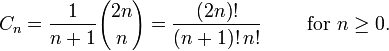
\includegraphics[scale=.6]{graphics/3bd4ac77a4af3f894d8e88ed7e1ba418.png}
% \caption{C\_n =
% \textbackslash{}frac\{1\}\{n+1\}\{2n\textbackslash{}choose n\} =
% \textbackslash{}frac\{(2n)!\}\{(n+1)!\textbackslash{},n!\}
% \textbackslash{}qquad\textbackslash{}mbox\{ for \}n\textbackslash{}ge
% 0.}
\end{figure}

Or recursively:

\begin{figure}[htbp]
\centering
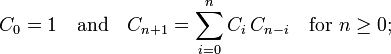
\includegraphics[scale=.6]{graphics/2f17435a71394ce667ab694b27341560.png}
% \caption{C\_0 = 1 \textbackslash{}quad \textbackslash{}mbox\{and\}
% \textbackslash{}quad
% C\_\{n+1\}=\textbackslash{}sum\_\{i=0\}\^{}\{n\}C\_i\textbackslash{},C\_\{n-i\}\textbackslash{}quad\textbackslash{}text\{for
% \}n\textbackslash{}ge 0;}
\end{figure}

Or alternatively (also recursive):

\begin{figure}[htbp]
\centering
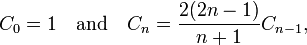
\includegraphics[scale=.6]{graphics/619a49e5557ce15be15ecd45dc767c72.png}
% \caption{C\_0 = 1 \textbackslash{}quad \textbackslash{}mbox\{and\}
% \textbackslash{}quad
% C\_n=\textbackslash{}frac\{2(2n-1)\}\{n+1\}C\_\{n-1\},}
\end{figure}

Implement at least one of these algorithms and print out the first 15
Catalan numbers with each. \emph{Memoization} is not
required, but may be worth the effort when using the second method
above.

\begin{description}
\item[Cf.]
\end{description}

\begin{itemize}
\item
  \emph{Pascal's triangle}
\item
  \href{http://milan.milanovic.org/math/english/fibo/fibo4.html}{Catalan
  Numbers and the Pascal Triangle}
\item
  \href{http://rosettacode.org/wiki/Catalan\_numbers\#An\_Alternative\_Approach}{http://rosettacode.org/wiki/Catalan\_numbers\#An\_Alternative\_Approach}
\end{itemize}


\begin{wideverbatim}

# Factorial
(de fact (N)
   (if (=0 N)
      1
      (* N (fact (dec N))) ) )

# Directly
(de catalanDir (N)
   (/ (fact (* 2 N)) (fact (inc N)) (fact N)) )

# Recursively
(de catalanRec (N)
   (if (=0 N)
      1
      (cache '(NIL) (pack (char (hash N)) N)  # Memoize
         (sum
            '((I) (* (catalanRec I) (catalanRec (- N I 1))))
            (range 0 (dec N)) ) ) ) )

# Alternatively
(de catalanAlt (N)
   (if (=0 N)
      1
      (*/ 2 (dec (* 2 N)) (catalanAlt (dec N)) (inc N)) ) )

# Test
(for (N 0 (> 15 N) (inc N))
   (tab (2 4 8 8 8)
      N
      " => "
      (catalanDir N)
      (catalanRec N)
      (catalanAlt N) ) )

Output:

 0 =>        1       1       1
 1 =>        1       1       1
 2 =>        2       2       2
 3 =>        5       5       5
 4 =>       14      14      14
 5 =>       42      42      42
 6 =>      132     132     132
 7 =>      429     429     429
 8 =>     1430    1430    1430
 9 =>     4862    4862    4862
10 =>    16796   16796   16796
11 =>    58786   58786   58786
12 =>   208012  208012  208012
13 =>   742900  742900  742900
14 =>  2674440 2674440 2674440

\end{wideverbatim}

\pagebreak{}
\section*{Character codes}

Given a character value in your language, print its code (could be ASCII
code, Unicode code, or whatever your language uses). For example, the
character `a' (lowercase letter A) has a code of 97 in ASCII (as well as
Unicode, as ASCII forms the beginning of Unicode). Conversely, given a
code, print out the corresponding character.


\begin{figure}[H]
  \centering
  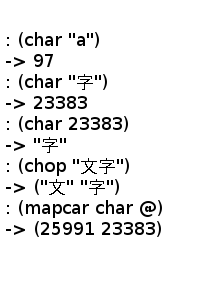
\includegraphics[scale=.6]{graphics/kanji.png}
\end{figure}

% \begin{CJK}{UTF8}{}
% \begin{Japanese}
% \noindent: (char ``a'') \\
% -> 97 \\
% : (char ``字'') \\
% -> 23383 \\
% : (char 23383) \\
% -> ``字'' \\
% : (chop ``文字'') \\
% -> (``文'' ``字'') \\
% : (mapcar char @) \\
% -> (25991 23383)
% \end{Japanese}
% \end{CJK}

% \begin{wideverbatim}

% : (char "a")
% -> 97
% : (char "字")
% -> 23383
% : (char 23383)
% -> "字"
% : (chop "文字")
% -> ("文" "字")
% : (mapcar char @)
% -> (25991 23383)

% \end{wideverbatim}

\pagebreak{}
\section*{Character matching}


\textbf{Basic Data Operation}\\ This is a basic data operation. It
represents a fundamental action on a basic data type.

You may see other such operations in the \emph{Basic Data Operations}
category, or:

\textbf{Integer Operations} \\
\emph{Arithmetic} \textbar{} \emph{Comparison}

\textbf{Boolean Operations} \\ \emph{Bitwise} \textbar{}
\emph{Logical}

\textbf{String Operations} \\
\emph{Concatenation} \textbar{} \emph{Interpolation} \textbar{}
\textbf{Matching}

\textbf{Memory Operations} \\
\emph{Pointers \& references} \textbar{} \emph{Addresses}

Given two strings, demonstrate the following 3 types of matchings:

\begin{enumerate}
\item
  Determining if the first string starts with second string
\item
  Determining if the first string contains the second string at any
  location
\item
  Determining if the first string ends with the second string
\end{enumerate}

Optional requirements:

\begin{enumerate}
\item
  Print the location of the match for part 2
\item
  Handle multiple occurrences of a string for part 2.
\end{enumerate}



\begin{wideverbatim}

: (pre? "ab" "abcd")
-> "abcd"
: (pre? "xy" "abcd")
-> NIL

: (sub? "bc" "abcd")
-> "abcd"
: (sub? "xy" "abcd")
-> NIL

: (tail (chop "cd") (chop "abcd"))
-> ("c" "d")
: (tail (chop "xy") (chop "abcd"))
-> NIL


(de positions (Pat Str)
   (setq Pat (chop Pat))
   (make
      (for ((I . L) (chop Str) L (cdr L))
         (and (head Pat L) (link I)) ) ) )

: (positions "bc" "abcdabcd")
-> (2 6)

\end{wideverbatim}

\pagebreak{}
\section*{Chat server}

Write a server for a minimal text based chat. People should be able to
connect via `telnet', sign on with a nickname, and type messages which
will then be seen by all other connected users. Arrivals and departures
of chat members should generate appropriate notification messages.



\begin{wideverbatim}

#!/usr/bin/picolisp /usr/lib/picolisp/lib.l
 
(de chat Lst
   (out *Sock
      (mapc prin Lst)
      (prinl) ) )
 
(setq *Port (port 4004))
 
(loop
   (setq *Sock (listen *Port))
   (NIL (fork) (close *Port))
   (close *Sock) )
 
(out *Sock
   (prin "Please enter your name: ")
   (flush) )
(in *Sock (setq *Name (line T)))
 
(tell 'chat "+++ " *Name " arrived +++")
 
(task *Sock
   (in @
      (ifn (eof)
         (tell 'chat *Name "> " (line T))
         (tell 'chat "--- " *Name " left ---")
         (bye) ) ) )
(wait)

\end{wideverbatim}

\begin{wideverbatim}

Output:

After starting the above script, connect to the chat server from two terminals:

           Terminal 1            |           Terminal 2
---------------------------------+---------------------------------
\$ telnet localhost 4004         |
Trying ::1...                    |
Trying 127.0.0.1...              |
Connected to localhost.          |
Escape character is '^]'.        |
Please enter your name: Ben      |
                                 | \$ telnet localhost 4004
                                 | Trying ::1...
                                 | Trying 127.0.0.1...
                                 | Connected to localhost.
                                 | Escape character is '^]'.
                                 | Please enter your name: Tom
+++ Tom arrived +++              |
Hi Tom                           |
                                 | Ben> Hi Tom
                                 | Hi Ben
Tom> Hi Ben                      |
                                 | How are you?
Tom> How are you?                |
Thanks, fine!                    |
                                 | Ben> Thanks, fine!
                                 | See you!
Tom> See you!                    |
                                 | ^]
                                 | telnet> quit
--- Tom left ---                 |
                                 | Connection closed.
                                 | \$

\end{wideverbatim}

\pagebreak{}
\section*{Checkpoint synchronization}

The checkpoint synchronization is a problem of synchronizing multiple
\emph{tasks}. Consider a workshop where several workers (\emph{tasks})
assembly details of some mechanism. When each of them completes his
work they put the details together. There is no store, so a worker who
finished its part first must wait for others before starting another
one. Putting details together is the \emph{checkpoint} at which
\emph{tasks} synchronize themselves before going their paths apart.

\textbf{The task}

Implement checkpoint synchronization in your language.

Make sure that the solution is \emph{race condition}-free. Note that a
straightforward solution based on \emph{events} is exposed to
\emph{race condition}. Let two \emph{tasks} A and B need to be
synchronized at a checkpoint. Each signals its event (\emph{EA} and
\emph{EB} correspondingly), then waits for the AND-combination of the
events (\emph{EA}\&\emph{EB}) and resets its event. Consider the
following scenario: A signals \emph{EA} first and gets blocked waiting
for \emph{EA}\&\emph{EB}. Then B signals \emph{EB} and loses the
processor. Then A is released (both events are signaled) and resets
\emph{EA}. Now if B returns and enters waiting for
\emph{EA}\&\emph{EB}, it gets lost.

When a worker is ready it shall not continue before others finish. A
typical implementation bug is when a worker is counted twice within one
working cycle causing its premature completion. This happens when the
quickest worker serves its cycle two times while the laziest one is
lagging behind.

If you can, implement workers joining and leaving.

\begin{wideverbatim}

The following solution implements each worker as a coroutine. Therefore, it
works only in the 64-bit version.

'checkpoints' takes a number of projects to do, and a number of workers. Each
worker is started with a random number of steps to do (between 2 and 5), and is
kept in a list of 'Staff' members. Whenever a worker finishes, he is removed
from that list, until it is empty and the project is done.

'worker' takes a number of steps to perform. It "works" by printing each step,
and returning NIL when done.

(de checkpoints (Projects Workers)
   (for P Projects
      (prinl "Starting project number " P ":")
      (for
         (Staff
            (mapcar
               '((I) (worker (format I) (rand 2 5)))  # Create staff of workers
               (range 1 Workers) )
            Staff                                     # While still busy
            (filter worker Staff) ) )                 # Remove finished workers
      (prinl "Project number " P " is done.") ) )

(de worker (ID Steps)
   (co ID
      (prinl "Worker " ID " has " Steps " steps to do")
      (for N Steps
         (yield ID)
         (prinl "Worker " ID " step " N) )
      NIL ) )

\end{wideverbatim}

\begin{wideverbatim}

Output:

: (checkpoints 2 3)  # Start two projects with 3 workers
Starting project number 1:
Worker 1 has 2 steps to do
Worker 2 has 3 steps to do
Worker 3 has 5 steps to do
Worker 1 step 1
Worker 2 step 1
Worker 3 step 1
Worker 1 step 2
Worker 2 step 2
Worker 3 step 2
Worker 2 step 3
Worker 3 step 3
Worker 3 step 4
Worker 3 step 5
Project number 1 is done.
Starting project number 2:
Worker 1 has 4 steps to do
Worker 2 has 3 steps to do
Worker 3 has 2 steps to do
Worker 1 step 1
Worker 2 step 1
Worker 3 step 1
Worker 1 step 2
Worker 2 step 2
Worker 3 step 2
Worker 1 step 3
Worker 2 step 3
Worker 1 step 4
Project number 2 is done.

\end{wideverbatim}

\pagebreak{}
\section*{Chess player}

In the early times, chess used to be the prime example of artificial
intelligence. Nowadays, some chess programs can beat a human master, and
simple implementations can be written in a few pages of code.

Write a program which plays chess against a human player. No need for
graphics -- a textual user interface is sufficient.

\begin{wideverbatim}

See [[Chess player/PicoLisp]].

This implementation supports all chess rules (including castling, pawn promotion
and en passant), switching sides, unlimited undo/redo, and the setup, saving and
loading of board positions to/from files.


# *Board a1 .. h8
# *White *Black *WKPos *BKPos *Pinned
# *Depth *Moved *Undo *Redo *Me *You
 
(load "@lib/simul.l")

### Fields/Board ###
# x y color piece whAtt blAtt
 
(setq *Board (grid 8 8))
 
(for (X . Lst) *Board
   (for (Y . This) Lst
      (=: x X)
      (=: y Y)
      (=: color (not (bit? 1 (+ X Y)))) ) )
 
(de *Straight `west `east `south `north)
 
(de *Diagonal
   ((This) (: 0 1  1  0 -1  1))   # Southwest
   ((This) (: 0 1  1  0 -1 -1))   # Northwest
   ((This) (: 0 1 -1  0 -1  1))   # Southeast
   ((This) (: 0 1 -1  0 -1 -1)) ) # Northeast
 
(de *DiaStraight
   ((This) (: 0 1  1  0 -1  1  0 -1  1))   # South Southwest
   ((This) (: 0 1  1  0 -1  1  0  1  1))   # West Southwest
   ((This) (: 0 1  1  0 -1 -1  0  1  1))   # West Northwest
   ((This) (: 0 1  1  0 -1 -1  0 -1 -1))   # North Northwest
   ((This) (: 0 1 -1  0 -1 -1  0 -1 -1))   # North Northeast
   ((This) (: 0 1 -1  0 -1 -1  0  1 -1))   # East Northeast
   ((This) (: 0 1 -1  0 -1  1  0  1 -1))   # East Southeast
   ((This) (: 0 1 -1  0 -1  1  0 -1  1)) ) # South Southeast
 

\end{wideverbatim}

\begin{wideverbatim}
 
### Pieces ###
(de piece (Typ Cnt Fld)
   (prog1
      (def
         (pack (mapcar '((Cls) (cdr (chop Cls))) Typ))
         Typ )
      (init> @ Cnt Fld) ) )
 
 
(class +White)
# color ahead
 
(dm init> (Cnt Fld)
   (=: ahead north)
   (extra Cnt Fld) )
 
(dm name> ()
   (pack " " (extra) " ") )
 
(dm move> (Fld)
   (adjMove '*White '*WKPos whAtt- whAtt+) )
 
 
(class +Black)
# color ahead
 
(dm init> (Cnt Fld)
   (=: color T)
   (=: ahead south)
   (extra Cnt Fld) )
 
(dm name> ()
   (pack '< (extra) '>) )
 
(dm move> (Fld)
   (adjMove '*Black '*BKPos blAtt- blAtt+) )
 
 
(class +piece)
# cnt field attacks
 
(dm init> (Cnt Fld)
   (=: cnt Cnt)
   (move> This Fld) )
 
(dm ctl> ())
 

\end{wideverbatim}

\begin{wideverbatim}

 
(class +King +piece)
 
(dm name> () 'K)
 
(dm val> () 120)
 
(dm ctl> ()
   (unless (=0 (: cnt)) -10) )
 
(dm moves> ()
   (make
      (unless
         (or
            (n0 (: cnt))
            (get (: field) (if (: color) 'whAtt 'blAtt)) )
         (tryCastle west T)
         (tryCastle east) )
      (try1Move *Straight)
      (try1Move *Diagonal) ) )
 
(dm attacks> ()
   (make
      (try1Attack *Straight)
      (try1Attack *Diagonal) ) )
 
 
(class +Castled)
 
(dm ctl> () 30)
 
 
(class +Queen +piece)
 
(dm name> () 'Q)
 
(dm val> () 90)
 
(dm moves> ()
   (make
      (tryMoves *Straight)
      (tryMoves *Diagonal) ) )
 
(dm attacks> ()
   (make
      (tryAttacks *Straight)
      (tryAttacks *Diagonal T) ) )
 

\end{wideverbatim}

\begin{wideverbatim}

 
(class +Rook +piece)
 
(dm name> () 'R)
 
(dm val> () 47)
 
(dm moves> ()
   (make (tryMoves *Straight)) )
 
(dm attacks> ()
   (make (tryAttacks *Straight)) )
 
 
(class +Bishop +piece)
 
(dm name> () 'B)
 
(dm val> () 33)
 
(dm ctl> ()
   (when (=0 (: cnt)) -10) )
 
(dm moves> ()
   (make (tryMoves *Diagonal)) )
 
(dm attacks> ()
   (make (tryAttacks *Diagonal T)) )
 
 
(class +Knight +piece)
 
(dm name> () 'N)
 
(dm val> () 28)
 
(dm ctl> ()
   (when (=0 (: cnt)) -10) )
 
(dm moves> ()
   (make (try1Move *DiaStraight)) )
 
(dm attacks> ()
   (make (try1Attack *DiaStraight)) )


\end{wideverbatim}

\begin{wideverbatim}
 
 
(class +Pawn +piece)
 
(dm name> () 'P)
 
(dm val> () 10)
 
(dm moves> ()
   (let (Fld1 ((: ahead) (: field))  Fld2 ((: ahead) Fld1))
      (make
         (and
            (tryPawnMove Fld1 Fld2)
            (=0 (: cnt))
            (tryPawnMove Fld2 T) )
         (tryPawnCapt (west Fld1) Fld2 (west (: field)))
         (tryPawnCapt (east Fld1) Fld2 (east (: field))) ) ) )
 
(dm attacks> ()
   (let Fld ((: ahead) (: field))
      (make
         (and (west Fld) (link @))
         (and (east Fld) (link @)) ) ) )
 

\end{wideverbatim}

\begin{wideverbatim}
 
### Move Logic ###
(de inCheck (Color)
   (if Color (get *BKPos 'whAtt) (get *WKPos 'blAtt)) )
 
(de whAtt+ (This Pce)
   (=: whAtt (cons Pce (: whAtt))) )
 
(de whAtt- (This Pce)
   (=: whAtt (delq Pce (: whAtt))) )
 
(de blAtt+ (This Pce)
   (=: blAtt (cons Pce (: blAtt))) )
 
(de blAtt- (This Pce)
   (=: blAtt (delq Pce (: blAtt))) )
 
(de adjMove (Var KPos Att- Att+)
   (let (W (: field whAtt)  B (: field blAtt))
      (when (: field)
         (put @ 'piece NIL)
         (for F (: attacks) (Att- F This)) )
      (nond
         (Fld (set Var (delq This (val Var))))
         ((: field) (push Var This)) )
      (ifn (=: field Fld)
         (=: attacks)
         (put Fld 'piece This)
         (and (isa '+King This) (set KPos Fld))
         (for F (=: attacks (attacks> This)) (Att+ F This)) )
      (reAtttack W (: field whAtt) B (: field blAtt)) ) )
 
(de reAtttack (W W2 B B2)
   (for This W
      (unless (memq This W2)
         (for F (: attacks) (whAtt- F This))
         (for F (=: attacks (attacks> This)) (whAtt+ F This)) ) )
   (for This W2
      (for F (: attacks) (whAtt- F This))
      (for F (=: attacks (attacks> This)) (whAtt+ F This)) )
   (for This B
      (unless (memq This B2)
         (for F (: attacks) (blAtt- F This))
         (for F (=: attacks (attacks> This)) (blAtt+ F This)) ) )
   (for This B2
      (for F (: attacks) (blAtt- F This))
      (for F (=: attacks (attacks> This)) (blAtt+ F This)) ) )


\end{wideverbatim}

\begin{wideverbatim}

 
(de try1Move (Lst)
   (for Dir Lst
      (let? Fld (Dir (: field))
         (ifn (get Fld 'piece)
            (link (list This (cons This Fld)))
            (unless (== (: color) (get @ 'color))
               (link
                  (list This
                     (cons (get Fld 'piece))
                     (cons This Fld) ) ) ) ) ) ) )
 
(de try1Attack (Lst)
   (for Dir Lst
      (and (Dir (: field)) (link @)) )  )
 
(de tryMoves (Lst)
   (for Dir Lst
      (let Fld (: field)
         (loop
            (NIL (setq Fld (Dir Fld)))
            (T (get Fld 'piece)
               (unless (== (: color) (get @ 'color))
                  (link
                     (list This
                        (cons (get Fld 'piece))
                        (cons This Fld) ) ) ) )
            (link (list This (cons This Fld))) ) ) ) )
 
(de tryAttacks (Lst Diag)
   (use (Pce Cls Fld2)
      (for Dir Lst
         (let Fld (: field)
            (loop
               (NIL (setq Fld (Dir Fld)))
               (link Fld)
               (T
                  (and
                     (setq Pce (get Fld 'piece))
                     (<> (: color) (get Pce 'color)) ) )
               (T (== '+Pawn (setq Cls (last (type Pce))))
                  (and
                     Diag
                     (setq Fld2 (Dir Fld))
                     (= (get Fld2 'y) (get ((get Pce 'ahead) Fld) 'y))
                     (link Fld2) ) )
               (T (memq Cls '(+Knight +Queen +King)))
               (T (and Pce (xor Diag (== Cls '+Bishop)))) ) ) ) ) )



\end{wideverbatim}

\begin{wideverbatim}

 
(de tryPawnMove (Fld Flg)
   (unless (get Fld 'piece)
      (if Flg
         (link (list This (cons This Fld)))
         (for Cls '(+Queen +Knight +Rook +Bishop)
            (link
               (list This
                  (cons This)
                  (cons
                     (piece (list (car (type This)) Cls) (: cnt))
                     Fld ) ) ) ) ) ) )
 
(de tryPawnCapt (Fld1 Flg Fld2)
   (if (get Fld1 'piece)
      (unless (== (: color) (get @ 'color))
         (if Flg
            (link
               (list This
                  (cons (get Fld1 'piece))
                  (cons This Fld1) ) )
            (for Cls '(+Queen +Knight +Rook +Bishop)
               (link
                  (list This
                     (cons (get Fld1 'piece))
                     (cons This)
                     (cons
                        (piece (list (car (type This)) Cls) (: cnt))
                        Fld1 ) ) ) ) ) )
      (let? Pce (get Fld2 'piece)
         (and
            (== Pce (car *Moved))
            (= 1 (get Pce 'cnt))
            (isa '+Pawn Pce)
            (n== (: color) (get Pce 'color))
            (link (list This (cons Pce) (cons This Fld1))) ) ) ) )


\end{wideverbatim}

\begin{wideverbatim}
 
(de tryCastle (Dir Long)
   (use (Fld1 Fld2 Fld Pce)
      (or
         (get (setq Fld1 (Dir (: field))) 'piece)
         (get Fld1 (if (: color) 'whAtt 'blAtt))
         (get (setq Fld2 (Dir Fld1)  Fld Fld2) 'piece)
         (when Long
            (or
               (get (setq Fld (Dir Fld)) 'piece)
               (get Fld (if (: color) 'whAtt 'blAtt)) ) )
         (and
            (== '+Rook (last (type (setq Pce (get (Dir Fld) 'piece)))))
            (=0 (get Pce 'cnt))
            (link
               (list This
                  (cons This)
                  (cons
                     (piece (cons (car (type This)) '(+Castled +King)) 1)
                     Fld2 )
                  (cons Pce Fld1) ) ) ) ) ) )

(de pinned (Fld Lst Color)
   (use (Pce L P)
      (and
         (loop
            (NIL (setq Fld (Dir Fld)))
            (T (setq Pce (get Fld 'piece))
               (and
                  (= Color (get Pce 'color))
                  (setq L
                     (make
                        (loop
                           (NIL (setq Fld (Dir Fld)))
                           (link Fld)
                           (T (setq P (get Fld 'piece))) ) ) )
                  (<> Color (get P 'color))
                  (memq (last (type P)) Lst)
                  (cons Pce L) ) ) )
         (link @) ) ) )
 


\end{wideverbatim}

\begin{wideverbatim}

 
### Moves ###
# Move      ((p1 (p1 . f2))        . ((p1 . f1)))
# Capture   ((p1 (p2) (p1 . f2))   . ((p1 . f1) (p2 . f2)))
# Castle    ((K (K) (C . f2) (R . f4)) . ((R . f3) (K . f1)))
# Promote   ((P (P) (Q . f2))      . ((Q) (P . f1)))
# Capt/Prom ((P (p1) (P) (Q . f2)) . ((Q) (P . f1) (p1 . f2)))
(de moves (Color)
   (filter
      '((Lst)
         (prog2
            (move (car Lst))
            (not (inCheck Color))
            (move (cdr Lst)) ) )
      (mapcan
         '((Pce)
            (mapcar
               '((Lst)
                  (cons Lst
                     (flip
                        (mapcar
                           '((Mov) (cons (car Mov) (get Mov 1 'field)))
                           (cdr Lst) ) ) ) )
               (moves> Pce) ) )
         (if Color *Black *White) ) ) )
 
(de move (Lst)
   (if (atom (car Lst))
      (inc (prop (push '*Moved (pop 'Lst)) 'cnt))
      (dec (prop (pop '*Moved) 'cnt)) )
   (for Mov Lst
      (move> (car Mov) (cdr Mov)) ) )
 

\end{wideverbatim}

\begin{wideverbatim}

 
### Evaluation ###
(de mate (Color)
   (and (inCheck Color) (not (moves Color))) )
 
(de battle (Fld Prey Attacker Defender)
   (use Pce
      (loop
         (NIL (setq Pce (mini 'val> Attacker)) 0)
         (setq Attacker (delq Pce Attacker))
         (NIL (and (asoq Pce *Pinned) (not (memq Fld @)))
            (max 0 (- Prey (battle Fld (val> Pce) Defender Attacker))) ) ) ) )
 
# Ref. Sargon, Dan and Kate Spracklen, Hayden 1978
(de cost (Color)
   (if (mate (not Color))
      -9999
      (setq *Pinned
         (make
            (for Dir *Straight
               (pinned *WKPos '(+Rook +Queen))
               (pinned *BKPos '(+Rook +Queen) T) )
            (for Dir *Diagonal
               (pinned *WKPos '(+Bishop +Queen))
               (pinned *BKPos '(+Bishop +Queen) T) ) ) )
      (let (Ctl 0  Mat 0  Lose 0  Win1 NIL  Win2 NIL  Flg NIL)
         (use (White Black Col Same B)
            (for Lst *Board
               (for This Lst
                  (setq White (: whAtt)  Black (: blAtt))
                  ((if Color inc dec) 'Ctl (- (length White) (length Black)))
                  (let? Val (and (: piece) (val> @))
                     (setq Col (: piece color)  Same (== Col Color))
                     ((if Same dec inc) 'Ctl (ctl> (: piece)))
                     (unless
                        (=0
                           (setq B
                              (if Col
                                 (battle This Val White Black)
                                 (battle This Val Black White) ) ) )
                        (dec 'Val 5)
                        (if Same
                           (setq
                              Lose (max Lose B)
                              Flg (or Flg (== (: piece) (car *Moved))) )
                           (when (> B Win1)
                              (xchg 'B 'Win1)
                              (setq Win2 (max Win2 B)) ) ) )
                     ((if Same dec inc) 'Mat Val) ) ) ) )
         (unless (=0 Lose) (dec 'Lose 5))
         (if Flg
            (* 4 (+ Mat Lose))
            (when Win2
               (dec 'Lose (>> 1 (- Win2 5))) )
            (+ Ctl (* 4 (+ Mat Lose))) ) ) ) )

\end{wideverbatim}

\begin{wideverbatim}
 
### Game ###
(de display (Res)
   (when Res
      (disp *Board T
         '((This)
            (cond
               ((: piece) (name> @))
               ((: color) " - ")
               (T "   ") ) ) ) )
   (and (inCheck *You) (prinl "(+)"))
   Res )
 
(de moved? (Lst)
   (or
      (> 16 (length Lst))
      (find '((This) (n0 (: cnt))) Lst) ) )
 
(de bookMove (From To)
   (let Pce (get From 'piece)
      (list 0 (list (list Pce (cons Pce To)) (cons Pce From))) ) )
 
(de myMove ()
   (let? M
      (cadr
         (cond
            ((moved? (if *Me *Black *White))
               (game *Me *Depth moves move cost) )
            (*Me
               (if (member (get *Moved 1 'field 'x) (1 2 3 5))
                  (bookMove 'e7 'e5)
                  (bookMove 'd7 'd5) ) )
            ((rand T) (bookMove 'e2 'e4))
            (T (bookMove 'd2 'd4)) ) )
      (move (car (push '*Undo M)))
      (off *Redo)
      (cons
         (caar M)
         (cdr (asoq (caar M) (cdr M)))
         (pick cdr (cdar M)) ) ) )


\end{wideverbatim}

\begin{wideverbatim}

 
(de yourMove (From To Cls)
   (when
      (find
         '((Mov)
            (and
               (== (caar Mov) (get From 'piece))
               (== To (pick cdr (cdar Mov)))
               (or
                  (not Cls)
                  (isa Cls (car (last (car Mov)))) ) ) )
         (moves *You) )
      (prog1 (car (push '*Undo @))
         (off *Redo)
         (move @) ) ) )
 
(de undo ()
   (move (cdr (push '*Redo (pop '*Undo)))) )
 
(de redo ()
   (move (car (push '*Undo (pop '*Redo)))) )
 
(de setup (Depth You Init)
   (setq *Depth (or Depth 5)  *You You  *Me (not You))
   (off *White *Black *Moved *Undo *Redo)
   (for Lst *Board
      (for This Lst (=: piece) (=: whAtt) (=: blAtt)) )
   (if Init
      (for L Init
         (with (piece (cadr L) 0 (car L))
            (unless (caddr L)
               (=: cnt 1)
               (push '*Moved This) ) ) )
      (mapc
         '((Cls Lst)
            (piece (list '+White Cls) 0 (car Lst))
            (piece '(+White +Pawn) 0 (cadr Lst))
            (piece '(+Black +Pawn) 0 (get Lst 7))
            (piece (list '+Black Cls) 0 (get Lst 8)) )
         '(+Rook +Knight +Bishop +Queen +King +Bishop +Knight +Rook)
         *Board ) ) )


\end{wideverbatim}

\begin{wideverbatim}

 
(de main (Depth You Init)
   (setup Depth You Init)
   (display T) )
 
(de go Args
   (display
      (cond
         ((not Args) (xchg '*Me '*You) (myMove))
         ((== '- (car Args)) (and *Undo (undo)))
         ((== '+ (car Args)) (and *Redo (redo)))
         ((apply yourMove Args) (display T) (myMove)) ) ) )
 
# Print position to file
(de ppos (File)
   (out File
      (println
         (list 'main *Depth *You
            (lit
               (mapcar
                  '((This)
                     (list
                        (: field)
                        (val This)
                        (not (memq This *Moved)) ) )
                  (append *White *Black) ) ) ) ) ) )



\end{wideverbatim}

\begin{wideverbatim}


Start:

\$ pil chess.l -main +
   +---+---+---+---+---+---+---+---+
 8 |<R>|<N>|<B>|<Q>|<K>|<B>|<N>|<R>|
   +---+---+---+---+---+---+---+---+
 7 |<P>|<P>|<P>|<P>|<P>|<P>|<P>|<P>|
   +---+---+---+---+---+---+---+---+
 6 |   | - |   | - |   | - |   | - |
   +---+---+---+---+---+---+---+---+
 5 | - |   | - |   | - |   | - |   |
   +---+---+---+---+---+---+---+---+
 4 |   | - |   | - |   | - |   | - |
   +---+---+---+---+---+---+---+---+
 3 | - |   | - |   | - |   | - |   |
   +---+---+---+---+---+---+---+---+
 2 | P | P | P | P | P | P | P | P |
   +---+---+---+---+---+---+---+---+
 1 | R | N | B | Q | K | B | N | R |
   +---+---+---+---+---+---+---+---+
     a   b   c   d   e   f   g   h


\end{wideverbatim}

\begin{wideverbatim}

Entering moves:

: (go e2 e4)

Undo moves:

: (go -)

Redo:

: (go +)

Switch sides:

: (go)

Save position to a file:

: (ppos "file")

Load position from file:

: (load "file")

\end{wideverbatim}

\pagebreak{}
\section*{Cholesky decomposition}


Every symmetric, positive definite matrix A can be decomposed into a
product of a unique lower triangular matrix L and its transpose:

\emph{A} = \emph{L}\emph{L}\textsuperscript{\emph{T}}

\emph{L} is called- the \emph{Cholesky factor} of \emph{A}, and can be
interpreted as a generalized square root of \emph{A}, as described in
\href{http://en.wikipedia.org/wiki/Cholesky\_decomposition}{Cholesky
decomposition}.

In a 3x3 example, we have to solve the following system of equations:

\begin{figure}[H]
\centering
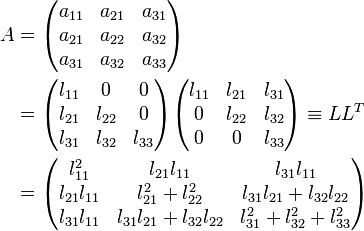
\includegraphics[scale=.6]{graphics/d9fa28df063d00917f713bd9de134ad5.png}
% \caption{\textbackslash{}begin\{align\} A \&=
% \textbackslash{}begin\{pmatrix\} a\_\{11\} \& a\_\{21\} \&
% a\_\{31\}\textbackslash{}\textbackslash{} a\_\{21\} \& a\_\{22\} \&
% a\_\{32\}\textbackslash{}\textbackslash{} a\_\{31\} \& a\_\{32\} \&
% a\_\{33\}\textbackslash{}\textbackslash{}
% \textbackslash{}end\{pmatrix\}\textbackslash{}\textbackslash{} \& =
% \textbackslash{}begin\{pmatrix\} l\_\{11\} \& 0 \& 0
% \textbackslash{}\textbackslash{} l\_\{21\} \& l\_\{22\} \& 0
% \textbackslash{}\textbackslash{} l\_\{31\} \& l\_\{32\} \&
% l\_\{33\}\textbackslash{}\textbackslash{} \textbackslash{}end\{pmatrix\}
% \textbackslash{}begin\{pmatrix\} l\_\{11\} \& l\_\{21\} \& l\_\{31\}
% \textbackslash{}\textbackslash{} 0 \& l\_\{22\} \& l\_\{32\}
% \textbackslash{}\textbackslash{} 0 \& 0 \& l\_\{33\}
% \textbackslash{}end\{pmatrix\} \textbackslash{}equiv
% LL\^{}T\textbackslash{}\textbackslash{} \&=
% \textbackslash{}begin\{pmatrix\} l\_\{11\}\^{}2 \& l\_\{21\}l\_\{11\} \&
% l\_\{31\}l\_\{11\} \textbackslash{}\textbackslash{} l\_\{21\}l\_\{11\}
% \& l\_\{21\}\^{}2 + l\_\{22\}\^{}2\&
% l\_\{31\}l\_\{21\}+l\_\{32\}l\_\{22\} \textbackslash{}\textbackslash{}
% l\_\{31\}l\_\{11\} \& l\_\{31\}l\_\{21\}+l\_\{32\}l\_\{22\} \&
% l\_\{31\}\^{}2 + l\_\{32\}\^{}2+l\_\{33\}\^{}2
% \textbackslash{}end\{pmatrix\}\textbackslash{}end\{align\} }
\end{figure}

We can see that for the diagonal elements
(\emph{l}\textsubscript{\emph{k}\emph{k}}) of \emph{L} there is a
calculation pattern:

\begin{figure}[H]
\centering
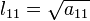
\includegraphics[scale=.6]{graphics/409b5a2625bed1a4a6c798323ae1db78.png}
% \caption{l\_\{11\} = \textbackslash{}sqrt\{a\_\{11\}\}}
\end{figure}

\begin{figure}[H]
\centering
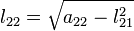
\includegraphics[scale=.6]{graphics/2cf603737e11dad8ec4d00dc8298c639.png}
% \caption{l\_\{22\} = \textbackslash{}sqrt\{a\_\{22\} - l\_\{21\}\^{}2\}}
\end{figure}

\begin{figure}[H]
\centering
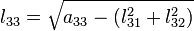
\includegraphics[scale=.6]{graphics/385714f276153424a4447fa0ede31bf4.png}
% \caption{l\_\{33\} = \textbackslash{}sqrt\{a\_\{33\} - (l\_\{31\}\^{}2 +
% l\_\{32\}\^{}2)\}}
\end{figure}

or in general:

\begin{figure}[H]
\centering
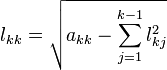
\includegraphics[scale=.6]{graphics/af307c5e65e7403b785f8a2c6b9d051a.png}
% \caption{l\_\{kk\} = \textbackslash{}sqrt\{a\_\{kk\} -
% \textbackslash{}sum\_\{j=1\}\^{}\{k-1\} l\_\{kj\}\^{}2\}}
\end{figure}

For the elements below the diagonal
(\emph{l}\textsubscript{\emph{i}\emph{k}}, where \emph{i} \textgreater{}
\emph{k}) there is also a calculation pattern:

\begin{figure}[H]
\centering
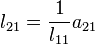
\includegraphics[scale=.6]{graphics/91035139969200d1af754ee0d07acd6a.png}
% \caption{l\_\{21\} = \textbackslash{}frac\{1\}\{l\_\{11\}\} a\_\{21\}}
\end{figure}

\begin{figure}[H]
\centering
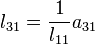
\includegraphics[scale=.6]{graphics/bdd8a535c6a8470767849ade18412c6d.png}
% \caption{l\_\{31\} = \textbackslash{}frac\{1\}\{l\_\{11\}\} a\_\{31\}}
\end{figure}

\begin{figure}[H]
\centering
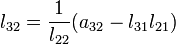
\includegraphics[scale=.6]{graphics/8c7f6df9ddc2c13f56a13ca113710587.png}
% \caption{l\_\{32\} = \textbackslash{}frac\{1\}\{l\_\{22\}\} (a\_\{32\} -
% l\_\{31\}l\_\{21\})}
\end{figure}

which can also be expressed in a general formula:

\begin{figure}[H]
\centering
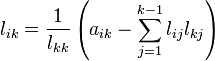
\includegraphics[scale=.6]{graphics/a404f9cdcc88e086294f604a41599f92.png}
% \caption{l\_\{ik\} = \textbackslash{}frac\{1\}\{l\_\{kk\}\}
% \textbackslash{}left ( a\_\{ik\} -
% \textbackslash{}sum\_\{j=1\}\^{}\{k-1\} l\_\{ij\}l\_\{kj\}
% \textbackslash{}right )}
\end{figure}

\textbf{Task description}

The task is to implement a routine which will return a lower Cholesky
factor \emph{L} for every given symmetric, positive definite nxn matrix
\emph{A}. You should then test it on the following two examples and
include your output.

Example 1:

\begin{wideverbatim}
25  15  -5                 5   0   0
15  18   0         -->     3   3   0
-5   0  11                -1   1   3
\end{wideverbatim}

Example 2:

\begin{wideverbatim}
18  22   54   42           4.24264    0.00000    0.00000    0.00000
22  70   86   62   -->     5.18545    6.56591    0.00000    0.00000
54  86  174  134          12.72792    3.04604    1.64974    0.00000
42  62  134  106           9.89949    1.62455    1.84971    1.39262
\end{wideverbatim}


\begin{wideverbatim}

(scl 9)
(load "@lib/math.l")

(de cholesky (A)
   (let L (mapcar '(() (need (length A) 0)) A)
      (for (I . R) A
         (for J I
            (let S (get R J)
               (for K (inc J)
                  (dec 'S (*/ (get L I K) (get L J K) 1.0)) )
               (set (nth L I J)
                  (if (= I J)
                     (sqrt (* 1.0 S))
                     (*/ S 1.0 (get L J J)) ) ) ) ) )
      (for R L
         (for N R (prin (align 9 (round N 5))))
         (prinl) ) ) )

Test:

(cholesky
   '((25.0 15.0 -5.0) (15.0 18.0 0) (-5.0 0 11.0)) )

(prinl)

(cholesky
   (quote
      (18.0  22.0   54.0   42.0)
      (22.0  70.0   86.0   62.0)
      (54.0  86.0  174.0  134.0)
      (42.0  62.0  134.0  106.0) ) )

Output:

  5.00000  0.00000  0.00000
  3.00000  3.00000  0.00000
 -1.00000  1.00000  3.00000

  4.24264  0.00000  0.00000  0.00000
  5.18545  6.56591  0.00000  0.00000
 12.72792  3.04604  1.64974  0.00000
  9.89949  1.62455  1.84971  1.39262

\end{wideverbatim}

\pagebreak{}
\section*{Classes}


In \emph{object-oriented programming} \textbf{class} is a set (a
\href{http://en.wikipedia.org/wiki/Transitive\_closure}{transitive
  closure}) of types bound by the relation of \emph{inheritance}. It
is said that all types derived from some base type T and the type T
itself form a class T. The first type T from the class T sometimes is
called the \textbf{root type} of the class.

A class of types itself, as a type, has the values and operations of
its own. The operations of are usually called \textbf{methods} of the
root type. Both operations and values are called \emph{polymorphic}.

A polymorphic operation (method) selects an implementation depending on
the actual specific type of the polymorphic argument. The action of
choice the type-specific implementation of a polymorphic operation is
called \textbf{dispatch}. Correspondingly, polymorphic operations are
often called \textbf{dispatching} or \textbf{virtual}. Operations with
multiple arguments and/or the results of the class are called
\textbf{multi-methods}. A further generalization of is the operation
with arguments and/or results from different classes.

\begin{itemize}
\item
  single-dispatch languages are those that allow only one argument or
  result to control the dispatch. Usually it is the first parameter,
  often hidden, so that a prefix notation \emph{x}.\emph{f}() is used
  instead of mathematical \emph{f}(\emph{x}).
\item
  multiple-dispatch languages allow many arguments and/or results to
  control the dispatch.
\end{itemize}

A polymorphic value has a type tag indicating its specific type from the
class and the corresponding specific value of that type. This type is
sometimes called \textbf{the most specific type} of a {[}polymorphic{]}
value. The type tag of the value is used in order to resolve the
dispatch. The set of polymorphic values of a class is a transitive
closure of the sets of values of all types from that class.

In many \emph{OO} languages the type of the class of T and T itself
are considered equivalent. In some languages they are distinct (like
in \emph{Ada}). When class T and T are equivalent, there is no way to
distinguish polymorphic and specific values.

The purpose of this task is to create a basic class with a method, a
constructor, an instance variable and how to instantiate it.


\begin{wideverbatim}

(class +Rectangle)
# dx dy

(dm area> ()  # Define a a method that calculates the rectangle's area
   (* (: dx) (: dy)) )

(println  # Create a rectangle, and print its area
   (area> (new '(+Rectangle) 'dx 3 'dy 4)) )

\end{wideverbatim}

\pagebreak{}
\section*{Closest-pair problem}

The aim of this task is to provide a function to find the closest two
points among a set of given points in two dimensions, i.e. to solve the
\href{http://en.wikipedia.org/wiki/Closest\_pair\_of\_points\_problem}{Closest
pair of points problem} in the \emph{planar} case.

The straightforward solution is a O(n\textsuperscript{2}) algorithm
(which we can call \emph{brute-force algorithm}); the pseudocode (using
indexes) could be simply:

\begin{wideverbatim}
bruteForceClosestPair of P(1), P(2), ... P(N)
if N < 2 then
  return ∞
else
  minDistance ← |P(1) - P(2)|
  minPoints ← { P(1), P(2) }
  foreach i ∈ [1, N-1]
    foreach j ∈ [i+1, N]
      if |P(i) - P(j)| < minDistance then
        minDistance ← |P(i) - P(j)|
        minPoints ← { P(i), P(j) } 
      endif
    endfor
  endfor
  return minDistance, minPoints
 endif
\end{wideverbatim}

A better algorithm is based on the recursive divide\&conquer approach,
as explained also at
\href{http://en.wikipedia.org/wiki/Closest\_pair\_of\_points\_problem\#Planar\_case}{Wikipedia},
which is O(\emph{n} log \emph{n}); a pseudocode could be:

\begin{wideverbatim}
closestPair of (xP, yP)
               where xP is P(1) .. P(N) sorted by x coordinate, and
                     yP is P(1) .. P(N) sorted by y coordinate (ascending order)
if N ≤ 3 then
  return closest points of xP using brute-force algorithm
else
  xL ← points of xP from 1 to ⌈N/2⌉
  xR ← points of xP from ⌈N/2⌉+1 to N
  xm ← xP(⌈N/2⌉)x
  yL ← { p ∈ yP : px ≤ xm }
  yR ← { p ∈ yP : px > xm }
  (dL, pairL) ← closestPair of (xL, yL)
  (dR, pairR) ← closestPair of (xR, yR)
  (dmin, pairMin) ← (dR, pairR)
  if dL < dR then
    (dmin, pairMin) ← (dL, pairL)
  endif
  yS ← { p ∈ yP : |xm - px| < dmin }
  nS ← number of points in yS
  (closest, closestPair) ← (dmin, pairMin)
  for i from 1 to nS - 1
    k ← i + 1
    while k ≤ nS and yS(k)y - yS(i)y < dmin
      if |yS(k) - yS(i)| < closest then
        (closest, closestPair) ← (|yS(k) - yS(i)|, {yS(k), yS(i)})
      endif
      k ← k + 1
    endwhile
  endfor
  return closest, closestPair
endif
\end{wideverbatim}

\textbf{References and further readings}

\begin{itemize}
\item
  \href{http://en.wikipedia.org/wiki/Closest\_pair\_of\_points\_problem}{Closest
  pair of points problem}
\item
  \href{http://www.cs.mcgill.ca/~cs251/ClosestPair/ClosestPairDQ.html}{Closest
  Pair (McGill)}
\item
  \href{http://www.cs.ucsb.edu/~suri/cs235/ClosestPair.pdf}{Closest Pair
  (UCSB)}
\item
  \href{http://classes.cec.wustl.edu/~cse241/handouts/closestpair.pdf}{Closest
  pair (WUStL)}
\item
  \href{http://www.cs.iupui.edu/~xkzou/teaching/CS580/Divide-and-conquer-closestPair.ppt}{Closest
  pair (IUPUI)}
\end{itemize}


\begin{wideverbatim}

A brute-force solution:

(de closestPairBF (Lst)
   (let Min T
      (use (Pt1 Pt2)
         (for P Lst
            (for Q Lst
               (or
                  (== P Q)
                  (>=
                     (setq N
                        (let (A (- (car P) (car Q))  B (- (cdr P) (cdr Q)))
                           (+ (* A A) (* B B)) ) )
                     Min )
                  (setq Min N  Pt1 P  Pt2 Q) ) ) )
         (list Pt1 Pt2 (sqrt Min)) ) ) )

Test:

: (scl 6)
-> 6

: (closestPairBF
   (quote
      (0.654682 . 0.925557)
      (0.409382 . 0.619391)
      (0.891663 . 0.888594)
      (0.716629 . 0.996200)
      (0.477721 . 0.946355)
      (0.925092 . 0.818220)
      (0.624291 . 0.142924)
      (0.211332 . 0.221507)
      (0.293786 . 0.691701)
      (0.839186 . 0.728260) ) )
-> ((891663 . 888594) (925092 . 818220) 77910)

\end{wideverbatim}

\pagebreak{}
\section*{Closures/Variable capture}

\textbf{Task:} Create a list of 10 functions, in the simplest manner
possible (anonymous functions are encouraged), such that the function at
index \emph{i} (you may choose to start \emph{i} from either 0 or 1),
when run, should return the square of the index, that is,
\emph{i}\textsuperscript{2}. Display the result of running any but the
last function, to demonstrate that the function indeed remembers its
value.

\textbf{Goal:} To demonstrate how to create a series of independent
closures based on the same template but maintain separate copies of the
variable closed over. In imperative languages, one would generally use a
loop with a mutable counter variable. For each function to maintain the
correct number, it has to capture the \emph{value} of the variable at
the time it was created, rather than just a reference to the variable,
which would have a different value by the time the function was run.


\begin{wideverbatim}

(setq FunList
   (make
      (for @N 10
         (link (curry (@N) () (* @N @N))) ) ) )

Test:

: ((get FunList 2))
-> 4

: ((get FunList 8))
-> 64

\end{wideverbatim}

\pagebreak{}
\section*{Collections}


Collections are abstractions to represent sets of values. In
statically-typed languages, the values are typically of a common data
type.

Create a collection, and add a few values to it.


\begin{wideverbatim}

The direct way in PicoLisp is a linear list (other possibilities could involve
[http://software-lab.de/doc/refI.html#idx index] trees or
[http://software-lab.de/doc/ref.html#symbol property] lists).

: (setq Lst (3 4 5 6))
-> (3 4 5 6)

: (push 'Lst 2)
-> 2

: (push 'Lst 1)
-> 1

: Lst
-> (1 2 3 4 5 6)

: (insert 4 Lst 'X)
-> (1 2 3 X 4 5 6)

\end{wideverbatim}

\pagebreak{}
\section*{Color of a screen pixel}


Get color information from an arbitrary pixel on the screen, such as the
current location of the mouse cursor. The mouse cursor may or may not
have to be active in a GUI created by your program. These functions are
OS related.


\begin{wideverbatim}

Using '[http://www.muquit.com/muquit/software/grabc/grabc.html grabc]'
as recommended in the C solution

(in '(grabc)
   (mapcar hex (cdr (line NIL 1 2 2 2))) )

Output:

73,61,205
-> (73 61 205)

\end{wideverbatim}

\pagebreak{}
\section*{Colour bars/Display}

The task is to display a series of vertical color bars across the width
of the display. The color bars should either use the system palette, or
the sequence of colors: Black, Red, Green, Blue, Magenta, Cyan, Yellow,
White.


\begin{wideverbatim}

(call 'clear)

(let Width (in '(tput cols) (read))
   (do (in '(tput lines) (read))
      (for B (range 0 7)
         (call 'tput 'setab B)
         (space (/ Width 8)) )
      (prinl) ) )

(call 'tput 'sgr0)   # reset

\end{wideverbatim}

\pagebreak{}
\section*{Colour pinstripe/Display}

The task is to create 1 pixel wide coloured vertical pinstripes with a
sufficient number of pinstripes to span the entire width of the graphics
display. The pinstripes should either follow the system palette sequence
or a sequence that includes Black, Red, Green, Blue, Magenta, Cyan,
Yellow, White.

After filling the top quarter of the display, we switch to a wider 2
pixel wide vertical pinstripe pattern. Halfway down the display we
switch to 3 pixel wide vertical pinstripe and then finally to a 4 pixels
wide vertical pinstripe for the last quarter of the display.


\begin{wideverbatim}

(de *Colors  # Black Red Green Blue Magenta Cyan Yellow White
   ((0 0 0) (255 0 0) (0 255 0) (0 0 255)
      (255 0 255) (0 255   255) (255 255 0) (255 255 255) .) )
 
(let Ppm  # Create PPM of 384 x 288 pixels
   (make
      (for N 4
         (let L
            (make
               (do (/ 384 N)
                  (let C (pop *Colors)
                     (do N (link C)) ) ) )
            (do 72 (link L)) ) ) )
   (out '(display)  # Pipe to ImageMagick
      (prinl "P6")  # NetPBM format
      (prinl (length (car Ppm)) " " (length Ppm))
      (prinl 255)
      (for Y Ppm (for X Y (apply wr X))) ) )

\end{wideverbatim}

\pagebreak{}
\section*{Colour pinstripe/Printer}


The task is to create 1 point wide colour vertical pinstripes with a
sufficient number of pinstripes to span the entire width of the colour
graphics printer. The pinstripes should alternate between each
individual cartridge ink and ink pair and black and white pinstripes
should be included. A typical pinstripe sequence woud be black, red,
green, blue, magenta, cyan, yellow, white.

After the first inch of printing, we switch to a wider 2 pixel wide
vertical pinstripe pattern. and to 3 point wide vertical for the next
inch, and then 4 point wide, etc. This trend continues for the entire
length of the page (or for 12 inches of run length in the case of a
printer using continuous roll stationery). After printing the test
pattern the page is ejected (or the test pattern is rolled clear of the
printer enclosure, in the case of continuous roll printers).

Note that it is an acceptable solution to use the smallest marks that
the language provides, rather than working at native printer resolution,
where this is not achievable from within the language.

Optionally, on systems where the printer resolution cannot be
determined, it is permissible to prompt the user for printer resolution,
and to calculate point size based on user input, enabling fractional
point sizes to be used.



\begin{wideverbatim}

(load "@lib/ps.l")

# Using circular lists for an endless supply of colors
#      (black  red  green blue magenta cyan yellow white)
(setq
   Red   (0    100    0     0    100    0    100   100 .)
   Green (0     0    100    0     0    100   100   100 .)
   Blue  (0     0     0    100   100   100    0    100 .) )

(call 'lpr
   (pdf "pinstripes"
      (a4)  # 595 x 842 dots
      (let (I 0  Step 1)
         (for X 595
            (color (car Red) (car Green) (car Blue)
               (vline X 0 842) )
            (when (= Step (inc 'I))
               (zero I)
               (pop 'Red)
               (pop 'Green)
               (pop 'Blue) )
            (when (=0 (\% X 72))  # 1 inch
               (zero I)
               (inc 'Step) ) ) )
      (page) ) )

\end{wideverbatim}

\pagebreak{}
\section*{Combinations}

Given non-negative integers \texttt{m} and \texttt{n}, generate all
size \texttt{m}
\href{http://mathworld.wolfram.com/Combination.html}{combinations} of
the integers from 0 to \texttt{n-1} in sorted order (each combination
is sorted and the entire table is sorted).

For example, \texttt{3 comb 5} is

\begin{verbatim}
0 1 2
0 1 3
0 1 4
0 2 3
0 2 4
0 3 4
1 2 3
1 2 4
1 3 4
2 3 4
\end{verbatim}

If it is more ``natural'' in your language to start counting from
\texttt{1} instead of \texttt{0} the combinations can be of the integers
from \texttt{1} to \texttt{n}.


\begin{wideverbatim}

(de comb (M Lst)
   (cond
      ((=0 M) '(NIL))
      ((not Lst))
      (T
         (conc
            (mapcar
               '((Y) (cons (car Lst) Y))
               (comb (dec M) (cdr Lst)) )
            (comb M (cdr Lst)) ) ) ) )

(comb 3 (1 2 3 4 5))

\end{wideverbatim}

\pagebreak{}
\section*{Combinations with repetitions}

The set of combinations with repetitions is computed from a set,
\emph{S} (of cardinality \emph{n}), and a size of resulting selection,
\emph{k}, by reporting the sets of cardinality \emph{k} where each
member of those sets is chosen from \emph{S}. In the real world, it is
about choosing sets where there is a ``large'' supply of each type of
element and where the order of choice does not matter. For example:

Q: How many ways can a person choose two doughnuts from a store selling
three types of doughnut: iced, jam, and plain? (i.e., \emph{S} is
\{iced,jam,plain\}, \textbar{} \emph{S} \textbar{} = 3, and \emph{k} =
2.)

A: 6: \{iced, iced\}; \{iced, jam\}; \{iced, plain\}; \{jam, jam\};
\{jam, plain\}; \{plain, plain\}.

Note that both the order of items within a pair, and the order of the
pairs given in the answer is not significant; the pairs represent
multisets.

\textbf{Task description}

\begin{itemize}
\item
  Write a function/program/routine/.. to generate all the combinations
  with repetitions of \emph{n} types of things taken \emph{k} at a time
  and use it to \emph{show} an answer to the doughnut example above.
\item
  For extra credit, use the function to compute and show \emph{just the
  number of ways} of choosing three doughnuts from a choice of ten types
  of doughnut. Do not show the individual choices for this part.
\end{itemize}

\textbf{References:}

\begin{itemize}
\item
  \href{http://en.wikipedia.org/wiki/Combination}{k-combination with
  repetitions}
\end{itemize}


\begin{wideverbatim}

(de combrep (N Lst)
   (cond
      ((=0 N) '(NIL))
      ((not Lst))
      (T
         (conc
            (mapcar
               '((X) (cons (car Lst) X))
               (combrep (dec N) Lst) )
            (combrep N (cdr Lst)) ) ) ) )

Output:

: (combrep 2 '(iced jam plain))
-> ((iced iced) (iced jam) (iced plain) (jam jam) (jam plain) (plain plain))

: (length (combrep 3 (range 1 10)))
-> 220

\end{wideverbatim}

\pagebreak{}
\section*{Command-line arguments}


\textbf{Command-line arguments} is part of \emph{Short Circuit}'s
\textbf{\emph{Console Program Basics}} selection.

Retrieve the list of command-line arguments given to the program. For
programs that only print the arguments when run directly, see
\emph{Scripted main}.

See also \emph{Program name}.

For parsing command line arguments intelligently, see \emph{Parsing
  command-line arguments}.

Example command line:

\begin{verbatim}
myprogram -c "alpha beta" -h "gamma"
\end{verbatim}



\begin{wideverbatim}

There are three ways to handle command-line arguments in PicoLisp:

1. Obtain all arguments as a list of strings via 
'[http://software-lab.de/doc/refA.html#argv argv]'

2. Fetch each argument individually with 
'[http://software-lab.de/doc/refO.html#opt opt]'

3. Use the built-in 
[http://software-lab.de/doc/ref.html#invoc command-line interpretation], 
where arguments starting with a hypen are executed as functions.

Here we use the third option, as it is not so obvious, sometimes more flexible,
and in fact the most commonly used one for application development.

We define 'c' and 'h' as functions, which retrieve their argument with 'opt',
and then '[http://software-lab.de/doc/refL.html#load load]' all remaining
command line arguments.

#!/usr/bin/picolisp /usr/lib/picolisp/lib.l

(de c ()
   (prinl "Got 'c': " (opt)) )

(de h ()
   (prinl "Got 'h': " (opt)) )

(load T)
(bye)

Output:

\$ ./myprogram -c "alpha beta" -h "gamma"
Got 'c': alpha beta
Got 'h': gamma

\end{wideverbatim}

\pagebreak{}
\section*{Comments}

Demonstrate all ways to include text in a language source file which is
completely ignored by the compiler or interpreter.

\textbf{See Also:}\\

\begin{itemize}
\item
  \href{http://xkcd.com/156}{xkcd} (Humor: hand gesture denoting
  \texttt{//} for ``commenting out'' people).
\end{itemize}


\begin{wideverbatim}

# The rest of the line is ignored
#{
   This is a
   multiline comment
}#
NIL
Immediately stop reading this file. Because all text in the input file following
a top-level 'NIL' is ignored.

This is typically used conditionally, with a read-macro expression like
`*Dbg
so that this text is only read if in debugging mode.

\end{wideverbatim}

\pagebreak{}
\section*{Compile-time calculation}

Some programming languages allow calculation of values at compile time.
For this task, calculate 10! at compile time. Print the result when the
program is run.

Discuss what limitations apply to compile-time calculations in your
language.


\begin{wideverbatim}

The PicoLisp "compiler" is the so-called "reader", which converts the
human-readable source code into nested internal pointer structures. When it
runs, arbitrary expressions can be executed with the backqoute and tilde
operators ([http://software-lab.de/doc/ref.html#macro-io read macros]).

(de fact (N)
   (apply * (range 1 N)) )

(de foo ()
   (prinl "The value of fact(10) is " `(fact 10)) )

Output:

: (pp 'foo)  # Pretty-print the function
(de foo NIL
   (prinl "The value of fact(10) is " 3628800) )
-> foo

: (foo)  # Execute it
The value of fact(10) is 3628800
-> 3628800

\end{wideverbatim}

\pagebreak{}
\section*{Compound data type}

\textbf{Data Structure}\\ This illustrates a data structure, a means of
storing data within a program.

You may see other such structures in the \emph{Data Structures}
category.

Create a compound data type Point(x,y).

A compound data type is one that holds multiple independent values.
See also \emph{Enumeration}.



\begin{wideverbatim}

(class +Point)

(dm T (X Y)
   (=: x X)
   (=: y Y) )

(setq P (new '(+Point) 3 4))

(show P)

Output:

\$52717735311266 (+Point)
   y 4
   x 3

\end{wideverbatim}

\pagebreak{}
\section*{Concurrent computing}

Using either native language concurrency syntax or freely available
libraries write a program to display the strings ``Enjoy'' ``Rosetta''
``Code'', one string per line, in random order. Concurrency syntax
must use \emph{threads}, tasks, co-routines, or whatever concurrency
is called in your language.

\begin{wideverbatim}

Using background tasks

(for (N . Str) '("Enjoy" "Rosetta" "Code")
   (task (- N) (rand 1000 4000)              # Random start time 1 .. 4 sec
      Str Str                                # Closure with string value
      (println Str)                          # Task body: Print the string
      (task @) ) )                           # and stop the task

Using child processes

(for Str '("Enjoy" "Rosetta" "Code")
   (let N (rand 1000 4000)                   # Randomize
      (unless (fork)                         # Create child process
         (wait N)                            # Wait 1 .. 4 sec
         (println Str)                       # Print string
         (bye) ) ) )                         # Terminate child process

\end{wideverbatim}

\pagebreak{}
\section*{Conditional structures}


\textbf{Control Structures}

These are examples of \emph{control structures}. You may also be
interested in:

\begin{itemize}
\item
  \textbf{Conditional structures}
\item
  \emph{Exceptions}
\item
  \emph{Flow-control structures}
\item
  \emph{Loops}
\end{itemize}

This page lists the conditional structures offered by different
programming languages. Common conditional structures are
\textbf{if-then-else} and \textbf{switch}.



\begin{wideverbatim}

(if (condition)                  # If the condition evaluates to non-NIL
   (then-do-this)                # Then execute the following expression
   (else-do-that)                # Else execute all other expressions
   (and-more) )

(ifn (condition)                 # If the condition evaluates to NIL
   (then-do-this)                # Then execute the following expression
   (else-do-that)                # Else execute all other expressions
   (and-more) )

(when (condition)                # If the condition evaluates to non-NIL
   (then-do-this)                # Then execute tall following expressions
   (and-more) )

(unless (condition)              # If the condition evaluates to NIL
   (then-do-this)                # Then execute all following expressions
   (and-more) )

(if2 (condition1) (condition2)   # If both conditions evaluate to non-NIL
   (expression-both)             # Then execute this expression
   (expression-first)            # Otherwise this for the first
   (expression-second)           # or this the second condition.
   (expression-none)             # If both are NIL, all following expressions
   (and-more) )

\end{wideverbatim}

\begin{wideverbatim}

(cond
   ((condition1)                 # If this condition evaluates to non-NIL
      (expression 1)             # Execute these expression(s)
      (more 1) )
   ((condition2)                 # Otherwise, if this evaluates to non-NIL
      (expression 2)             # Execute these expression(s)
      (more 2) )
   (T                            # If none evaluated to non-NIL
      (expression 1)             # Execute these expression(s)
      (more 1) )

(nond
   ((condition1)                 # If this condition evaluates to NIL
      (expression 1)             # Execute these expression(s)
      (more 1) )
   ((condition2)                 # Otherwise, if this evaluates to NIL
      (expression 2)             # Execute these expression(s)
      (more 2) )
   (NIL                          # If none evaluated to NIL
      (expression 1)             # Execute these expression(s)
      (more 1) )

(case (expression)               # Evaluate the expression
   (value1                       # If it is equal to, or member of, 'value1'
      (do-this1)                 # Execute these expression(s)
      (do-that1) )
   (value2                       # Else if it is equal to, or member of, 'value2'
      (do-this2)                 # Execute these expression(s)
      (do-that2) )
   (T                            # Else execute final expression(s)
      (do-something-else) ) )

\end{wideverbatim}

\pagebreak{}
\section*{Constrained Random Points on a Circle}


Generate 100 \textless{}x,y\textgreater{} coordinate pairs such that x
and y are integers sampled from the uniform distribution with the
condition that
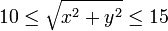
\includegraphics[scale=.6]{graphics/d8c852f6bb73b0d042422df261390347.png}.
Then display/plot them. The outcome should be a ``fuzzy'' circle. The
actual number of points plotted may be less than 100, given that some
pairs may be generated more than once.

There are several possible approaches to accomplish this. Here are two
possible algorithms.

1) Generate random pairs of integers and filter out those that don't
satisfy this condition:

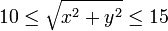
\includegraphics[scale=.6]{graphics/d8c852f6bb73b0d042422df261390347.png}.

2) Precalculate the set of all possible points (there are 404 of them)
and select randomly from this set.


\begin{wideverbatim}

(let Area (make (do 31 (link (need 31 " "))))
   (use (X Y)
      (do 100
         (until
            (>=
               15
               (sqrt
                  (+
                     (* (setq X (rand -15 15)) X)
                     (* (setq Y (rand -15 15)) Y) ) )
               10 ) )
         (set (nth Area (+ 16 X) (+ 16 Y)) "#") ) )
   (mapc prinl Area) )

Output:

           #
        ##
           #  #  #  #
         ## #    #  #   #
       #      #   # # #
    #       #     # #   #
      #   #         #    #
      #                #   #
                       #
       #               #
     ##                      #
                          #
   #                      # #
  ###                      #
 #                         # #
##                          # #
  #                        #
 #                        #
 ## #
                           #
   #
     #                 #
     #
   ###                  #   #
      ###           # #    #
    #      #
         #  #   ##
                 # #
      #     #           #
                # #  #

\end{wideverbatim}

\pagebreak{}
\section*{Constrained genericity}

\emph{Constrained genericity} means that a parametrized type or
function (see \emph{Parametric Polymorphism}) can only be instantiated
on types fulfilling some conditions, even if those conditions are not
used in that function.

Say a type is called ``eatable'' if you can call the function
\texttt{eat} on it. Write a generic type \texttt{FoodBox} which contains
a collection of objects of a type given as parameter, but can only be
instantiated on eatable types. The FoodBox shall not use the function
eat in any way (i.e. without the explicit restriction, it could be
instantiated on any type). The specification of a type being eatable
should be as generic as possible in your language (i.e. the restrictions
on the implementation of eatable types should be as minimal as
possible). Also explain the restrictions, if any, on the implementation
of eatable types, and show at least one example of an eatable type.



\begin{wideverbatim}

(class +Eatable)

(dm eat> ()
   (prinl "I'm eatable") )


(class +FoodBox)
# obj

(dm set> (Obj)
   (unless (method 'eat> Obj)                # Check if the object is eatable
      (quit "Object is not eatable" Obj) )
   (=: obj Obj) )                            # If so, set the object


(let (Box (new '(+FoodBox))  Eat (new '(+Eatable))  NoEat (new '(+Bla)))
   (set> Box Eat)       # Works
   (set> Box NoEat) )   # Gives an error

Output:

\$384320489 -- Object is not eatable

? (show Box)
\$384320487 (+FoodBox)
   obj \$384320488

? (show Box 'obj)
\$384320488 (+Eatable)

? (show NoEat)
\$384320489 (+Bla)

\end{wideverbatim}

\pagebreak{}
\section*{Conway's Game of Life}

The \textbf{Game of Life} is a
\href{http://en.wikipedia.org/wiki/cellular\_automaton}{cellular
  automaton} devised by the British mathematician
\href{http://en.wikipedia.org/wiki/John\_Horton\_Conway}{John Horton
  Conway} in 1970. It is the best-known example of a cellular
automaton.

Conway's game of life is described
\href{http://en.wikipedia.org/wiki/Conway\%27s\_Game\_of\_Life}{here}:

A cell \textbf{C} is represented by a 1 when alive or 0 when dead, in an
m-by-m square array of cells. We calculate \textbf{N} - the sum of live
cells in C's
\href{http://en.wikipedia.org/wiki/Moore\_neighborhood}{eight-location
neighbourhood}, then cell C is alive or dead in the next generation
based on the following table:

\begin{wideverbatim}
   C   N                 new C
   1   0,1             ->  0  # Lonely
   1   4,5,6,7,8       ->  0  # Overcrowded
   1   2,3             ->  1  # Lives
   0   3               ->  1  # It takes three to give birth!
   0   0,1,2,4,5,6,7,8 ->  0  # Barren
\end{wideverbatim}

Assume cells beyond the boundary are always dead.

The ``game'' is actually a zero-player game, meaning that its evolution
is determined by its initial state, needing no input from human players.
One interacts with the Game of Life by creating an initial configuration
and observing how it evolves.

Although you should test your implementation on more complex examples
such as the
\href{http://en.wikipedia.org/wiki/Conway\%27s\_Game\_of\_Life\#Examples\_of\_patterns}{glider}
in a larger universe, show the action of the blinker (three adjoining
cells in a row all alive), over three generations, in a 3 by 3 grid.



\begin{wideverbatim}

This example uses 'grid' and 'disp' from "lib/simul.l". These functions
maintain an array of multiply linked objects, and are also used in the chess
program and other games in the distribution.

(load "@lib/simul.l")
 
(de life (DX DY . Init)
   (let Grid (grid DX DY)
      (for This Init
         (=: life T) )
      (loop
         (disp Grid NIL
            '((This) (if (: life) "X " "  ")) )
         (wait 1000)
         (for Col Grid
            (for This Col
               (let N  # Count neighbors
                  (cnt
                     '((Dir) (get (Dir This) 'life))
                     (quote
                        west east south north
                        ((X) (south (west X)))
                        ((X) (north (west X)))
                        ((X) (south (east X)))
                        ((X) (north (east X))) ) )
                  (=: next  # Next generation
                     (if (: life)
                        (>= 3 N 2)
                        (= N 3) ) ) ) ) )
         (for Col Grid  # Update
            (for This Col
               (=: life (: next)) ) ) ) ) )
 
(life 5 5  b3 c3 d3)

\end{wideverbatim}

\begin{wideverbatim}
Output:

 5
 4
 3   X X X
 2
 1
   a b c d e
 5
 4     X
 3     X
 2     X
 1
   a b c d e
 5
 4
 3   X X X
 2
 1
   a b c d e

\end{wideverbatim}

\pagebreak{}
\section*{Copy a string}

This task is about copying a string. Where it is relevant, distinguish
between copying the contents of a string versus making an additional
reference to an existing string.

\begin{wideverbatim}

(setq Str1 "abcdef")
(setq Str2 Str1)                       # Create a reference to that symbol
(setq Str3 (name Str1))                # Create new symbol with name "abcdef"

\end{wideverbatim}

\pagebreak{}
\section*{Count occurrences of a substring}

The task is to either create a function, or show a built-in function, to
count the number of non-overlapping occurrences of a substring inside a
string. The function should take two arguments: the first argument being
the string to search and the second a substring to be search for. It
should return an integer count.

\begin{wideverbatim}

print countSubstring("the three truths","th")
3

// do not count substrings that overlap with
// previously-counted substrings:

print countSubstring("ababababab","abab")
2

\end{wideverbatim}

The matching should yield the highest number of non-overlapping matches.
In general, this essentially means matching from left-to-right or
right-to-left.


\begin{wideverbatim}

(de countSubstring (Str Sub)
   (let (Cnt 0  H (chop Sub))
      (for (S (chop Str)  S  (cdr S))
         (when (head H S)
            (inc 'Cnt)
            (setq S (map prog2 H S)) ) )
      Cnt ) )

Test:

: (countSubstring "the three truths" "th")
-> 3

: (countSubstring "ababababab" "abab")
-> 2

\end{wideverbatim}

\pagebreak{}
\section*{Count the Coins}


There are four types of common coins in US currency: quarters (25
cents), dimes (10), nickels (5) and pennies (1). There are 6 ways to
make change for 15 cents:

\begin{itemize}
\item
  A dime and a nickel;
\item
  A dime and 5 pennies;
\item
  3 nickels;
\item
  2 nickels and 5 pennies;
\item
  A nickel and 10 pennies;
\item
  15 pennies.
\end{itemize}

How many ways are there to make change for a dollar using these common
coins? (1 dollar = 100 cents).

\textbf{Optional:}

Less common are dollar coins (100 cents); very rare are half dollars (50
cents). With the addition of these two coins, how many ways are there to
make change for \$1000? (note: the answer is larger than
2\textsuperscript{32}).

\textbf{Algorithm}: See

\href{http://mitpress.mit.edu/sicp/full-text/book/book-Z-H-11.html\#\%\_sec\_Temp\_52}{http://mitpress.mit.edu/sicp/full-text/book/book-Z-H-11.html\#\%\_sec\_Temp\_52}.


\begin{wideverbatim}

(de coins (Sum Coins)
   (let (Buf (mapcar '((N) (cons 1 (need (dec N) 0))) Coins)  Prev)
      (do Sum
         (zero Prev)
         (for L Buf
            (inc (rot L) Prev)
            (setq Prev (car L)) ) )
      Prev ) )

Test:

(for Coins '((100 50 25 10 5 1) (200 100 50 20 10 5 2 1))
   (println (coins 100 (cddr Coins)))
   (println (coins (* 1000 100) Coins))
   (println (coins (* 10000 100) Coins))
   (println (coins (* 100000 100) Coins))
   (prinl) )

Output:

242
13398445413854501
1333983445341383545001
133339833445334138335450001

4562
10056050940818192726001
99341140660285639188927260001
992198221207406412424859964272600001

\end{wideverbatim}

\pagebreak{}
\section*{Counting in Factors}

Write a program which counts up from 1, displaying each number as the
multiplication of its prime factors. For the purpose of this task, 1 may
be shown as itself.

For examle, 2 is prime, so it would be shown as itself. 6 is not prime;
it would be shown as

\includegraphics[scale=.6]{graphics/4b3a89ff7af9ad06700897f831201197.png}.

Likewise, 2144 is not prime; it would be shown as

\includegraphics[scale=.6]{graphics/eae4d1b7a3788fd85e5c4995efc7e196.png}.

c.f. \emph{Prime decomposition}, \emph{Category:Prime\_Numbers}


\begin{wideverbatim}

This is the 'factor' function from [[Prime decomposition#PicoLisp]].

(de factor (N)
   (make
      (let (D 2  L (1 2 2 . (4 2 4 2 4 6 2 6 .))  M (sqrt N))
         (while (>= M D)
            (if (=0 (\% N D))
               (setq M (sqrt (setq N (/ N (link D)))))
               (inc 'D (pop 'L)) ) )
         (link N) ) ) )

(for N 20
   (prinl N ": " (glue " * " (factor N))) )

Output:

1: 1
2: 2
3: 3
4: 2 * 2
5: 5
6: 2 * 3
7: 7
8: 2 * 2 * 2
9: 3 * 3
10: 2 * 5
11: 11
12: 2 * 2 * 3
13: 13
14: 2 * 7
15: 3 * 5
16: 2 * 2 * 2 * 2
17: 17
18: 2 * 3 * 3
19: 19
20: 2 * 2 * 5

\end{wideverbatim}

\pagebreak{}
\section*{Counting in octal}

The task is to produce a sequential count in octal, starting at zero,
and using an increment of a one for each consecutive number. Each number
should appear on a single line, and the program should count until
terminated, or until the maximum value of the numeric type in use is
reached.

\begin{itemize}
\item \emph{Integer sequence} is a similar task without the use of
  octal numbers.
\end{itemize}


\begin{wideverbatim}

(for (N 0  T  (inc N))
   (prinl (oct N)) )

\end{wideverbatim}

\pagebreak{}
\section*{Create a file}

In this task, the job is to create a new empty file called
``output.txt'' of size 0 bytes and an empty directory called ``docs''.
This should be done twice: once ``here'', i.e. in the current working
directory and once in the filesystem root.


\begin{wideverbatim}

(out "output.txt")                     # Empty output
(call 'mkdir "docs")                   # Call external
(out "/output.txt")
(call 'mkdir "/docs")

\end{wideverbatim}

\pagebreak{}
\section*{Create a two-dimensional array at runtime}


\textbf{Data Structure}\\ This illustrates a data structure, a means of
storing data within a program.

You may see other such structures in the \emph{Data Structures}
category.

Get two integers from the user, then create a two-dimensional array
where the two dimensions have the sizes given by those numbers, and
which can be accessed in the most natural way possible. Write some
element of that array, and then output that element. Finally destroy
the array if not done by the language itself.


\begin{wideverbatim}

(de 2dimTest (DX DY)
   (let A (make (do DX (link (need DY))))
      (set (nth A 3 3) 999)            # Set A[3][3] to 999
      (mapc println A)                 # Print all
      (get A 3 3) ) )                  # Return A[3][3]

(2dimTest 5 5)

Output:

(NIL NIL NIL NIL NIL)
(NIL NIL NIL NIL NIL)
(NIL NIL 999 NIL NIL)
(NIL NIL NIL NIL NIL)
(NIL NIL NIL NIL NIL)
-> 999

\end{wideverbatim}

\pagebreak{}
\section*{Create an HTML table}


Create an HTML table.

\begin{itemize}
\item
  The table body should have at least three rows of three columns.
\item
  Each of these three columns should be labelled ``X'', ``Y'', and
  ``Z''.
\item
  An extra column should be added at either the extreme left or the
  extreme right of the table that has no heading, but is filled with
  sequential row numbers.
\item
  The rows of the ``X'', ``Y'', and ``Z'' columns should be filled with
  random or sequential integers having 4 digits or less.
\item
  The numbers should be aligned in the same fashion for all columns.
\end{itemize}



\begin{wideverbatim}

(load "@lib/xhtml.l")

(<table> NIL NIL '(NIL (NIL "X") (NIL "Y") (NIL "Z"))
   (for N 3
      (<row> NIL N 124 456 789) ) )

\end{wideverbatim}

\pagebreak{}
\section*{Create an object at a given address}


\textbf{Basic Data Operation}\\ This is a basic data operation. It
represents a fundamental action on a basic data type.

You may see other such operations in the \emph{Basic Data Operations}
category, or:

\textbf{Integer Operations} \\
\emph{Arithmetic} \textbar{} \emph{Comparison}

\textbf{Boolean Operations} \\ \emph{Bitwise} \textbar{}
\emph{Logical}

\textbf{String Operations} \\
\emph{Concatenation} \textbar{} \emph{Interpolation} \textbar{}
\emph{Matching}

\textbf{Memory Operations} \\
\emph{Pointers \& references} \textbar{} \emph{Addresses}

In systems programing it is sometimes required to place language objects
at specific memory locations, like I/O registers, hardware interrupt
vectors etc.

\textbf{Task}

Show how language objects can be allocated at a specific machine
addresses.

Since most \emph{OSes} prohibit access to the physical memory if it is
not mapped by the application, as an example, rather than a physical
address, take the address of some existing object (using suitable
\emph{address operations} if necessary). For example, create an
integer object. Print the machine address of the object. Take the
address of the object and create another integer object at this
address. Print the value of this object to verify that it is same as
one of the origin. Change the value of the origin and verify it again.


\begin{wideverbatim}

: (setq IntSpace 12345)          # Integer
-> 12345

: (setq Address (adr 'IntSpace)) # Encoded machine address
-> -2969166782547

: (set (adr Address) 65535)      # Set this address to a new value
-> 65535

: IntSpace                       # Show the new value
-> 65535

\end{wideverbatim}

\pagebreak{}
\section*{CSV to HTML translation}


Consider a simplified CSV format where all rows are separated by a
newline and all columns are separated by commas. No commas are allowed
as field data, but the data may contain other characters and character
sequences that would normally be escaped when converted to HTML

The task is to create a function that takes a string representation of
the CSV data and returns a text string of an HTML table representing the
CSV data. Use the following data as the CSV text to convert, and show
your output.

Character,Speech

The multitude,The messiah! Show us the messiah!

Brians mother,\textless{}angry\textgreater{}Now you listen here! He's
not the messiah; he's a very naughty boy! Now go
away!\textless{}/angry\textgreater{}

The multitude,Who are you?

Brians mother,I'm his mother; that's who!

The multitude,Behold his mother! Behold his mother!

For extra credit, \emph{optionally} allow special formatting for the
first row of the table as if it is the tables header row (via
\textless{}thead\textgreater{} preferably; CSS if you must).



\begin{wideverbatim}

Simple solution

(load "@lib/http.l")

(in "text.csv"
   (<table> 'myStyle NIL NIL
      (prinl)
      (while (split (line) ",")
         (<row> NIL (ht:Prin (pack (car @))) (ht:Prin (pack (cadr @))))
         (prinl) ) ) )

Output:

<table class="myStyle">
<tr><td>Character</td><td>Speech</td></tr>
<tr><td>The multitude</td><td>The messiah! Show us the messiah!</td></tr>
<tr><td>Brians mother</td><td>\&lt;angry\&gt;Now you listen here! 
He's not the messiah; he's a very naughty boy! Now go away!\&lt;/angry\&gt;</td></tr>
<tr><td>The multitude</td><td>Who are you?</td></tr>
<tr><td>Brians mother</td><td>I'm his mother; that's who!</td></tr>
<tr><td>The multitude</td><td>Behold his mother! Behold his mother!</td></tr>
</table>

Extra credit solution

(load "@lib/http.l")

(in "text.csv"
   (when (split (line) ",")
      (<table> 'myStyle NIL (mapcar '((S) (list NIL (pack S))) @)
         (prinl)
         (while (split (line) ",")
            (<row> NIL (ht:Prin (pack (car @))) (ht:Prin (pack (cadr @))))
            (prinl) ) ) ) )

Output:

<table class="myStyle"><tr><th>Character</th><th>Speech</th></tr>
<tr><td>The multitude</td><td>The messiah! Show us the messiah!</td></tr>
<tr><td>Brians mother</td><td>\&lt;angry\&gt;Now you listen here! 
He's not the messiah; he's a very naughty boy! Now go away!\&lt;/angry\&gt;</td></tr>
<tr><td>The multitude</td><td>Who are you?</td></tr>
<tr><td>Brians mother</td><td>I'm his mother; that's who!</td></tr>
<tr><td>The multitude</td><td>Behold his mother! Behold his mother!</td></tr>
</table>

\end{wideverbatim}


% %%%%%%%%%%%%%%%%%%%%%%%% referenc.tex %%%%%%%%%%%%%%%%%%%%%%%%%%%%%%
% sample references
% %
% Use this file as a template for your own input.
%
%%%%%%%%%%%%%%%%%%%%%%%% Springer-Verlag %%%%%%%%%%%%%%%%%%%%%%%%%%
%
% BibTeX users please use
% \bibliographystyle{}
% \bibliography{}
%
\biblstarthook{In view of the parallel print and (chapter-wise) online publication of your book at \url{www.springerlink.com} it has been decided that -- as a genreral rule --  references should be sorted chapter-wise and placed at the end of the individual chapters. However, upon agreement with your contact at Springer you may list your references in a single seperate chapter at the end of your book. Deactivate the class option \texttt{sectrefs} and the \texttt{thebibliography} environment will be put out as a chapter of its own.\\\indent
References may be \textit{cited} in the text either by number (preferred) or by author/year.\footnote{Make sure that all references from the list are cited in the text. Those not cited should be moved to a separate \textit{Further Reading} section or chapter.} The reference list should ideally be \textit{sorted} in alphabetical order -- even if reference numbers are used for the their citation in the text. If there are several works by the same author, the following order should be used: 
\begin{enumerate}
\item all works by the author alone, ordered chronologically by year of publication
\item all works by the author with a coauthor, ordered alphabetically by coauthor
\item all works by the author with several coauthors, ordered chronologically by year of publication.
\end{enumerate}
The \textit{styling} of references\footnote{Always use the standard abbreviation of a journal's name according to the ISSN \textit{List of Title Word Abbreviations}, see \url{http://www.issn.org/en/node/344}} depends on the subject of your book:
\begin{itemize}
\item The \textit{two} recommended styles for references in books on \textit{mathematical, physical, statistical and computer sciences} are depicted in ~\cite{science-contrib, science-online, science-mono, science-journal, science-DOI} and ~\cite{phys-online, phys-mono, phys-journal, phys-DOI, phys-contrib}.
\item Examples of the most commonly used reference style in books on \textit{Psychology, Social Sciences} are~\cite{psysoc-mono, psysoc-online,psysoc-journal, psysoc-contrib, psysoc-DOI}.
\item Examples for references in books on \textit{Humanities, Linguistics, Philosophy} are~\cite{humlinphil-journal, humlinphil-contrib, humlinphil-mono, humlinphil-online, humlinphil-DOI}.
\item Examples of the basic Springer style used in publications on a wide range of subjects such as \textit{Computer Science, Economics, Engineering, Geosciences, Life Sciences, Medicine, Biomedicine} are ~\cite{basic-contrib, basic-online, basic-journal, basic-DOI, basic-mono}. 
\end{itemize}
}

\begin{thebibliography}{99.}%
% and use \bibitem to create references.
%
% Use the following syntax and markup for your references if 
% the subject of your book is from the field 
% "Mathematics, Physics, Statistics, Computer Science"
%
% Contribution 
\bibitem{science-contrib} Broy, M.: Software engineering --- from auxiliary to key technologies. In: Broy, M., Dener, E. (eds.) Software Pioneers, pp. 10-13. Springer, Heidelberg (2002)
%
% Online Document
\bibitem{science-online} Dod, J.: Effective substances. In: The Dictionary of Substances and Their Effects. Royal Society of Chemistry (1999) Available via DIALOG. \\
\url{http://www.rsc.org/dose/title of subordinate document. Cited 15 Jan 1999}
%
% Monograph
\bibitem{science-mono} Geddes, K.O., Czapor, S.R., Labahn, G.: Algorithms for Computer Algebra. Kluwer, Boston (1992) 
%
% Journal article
\bibitem{science-journal} Hamburger, C.: Quasimonotonicity, regularity and duality for nonlinear systems of partial differential equations. Ann. Mat. Pura. Appl. \textbf{169}, 321--354 (1995)
%
% Journal article by DOI
\bibitem{science-DOI} Slifka, M.K., Whitton, J.L.: Clinical implications of dysregulated cytokine production. J. Mol. Med. (2000) doi: 10.1007/s001090000086 
%
\bigskip

% Use the following (APS) syntax and markup for your references if 
% the subject of your book is from the field 
% "Mathematics, Physics, Statistics, Computer Science"
%
% Online Document
\bibitem{phys-online} J. Dod, in \textit{The Dictionary of Substances and Their Effects}, Royal Society of Chemistry. (Available via DIALOG, 1999), 
\url{http://www.rsc.org/dose/title of subordinate document. Cited 15 Jan 1999}
%
% Monograph
\bibitem{phys-mono} H. Ibach, H. L\"uth, \textit{Solid-State Physics}, 2nd edn. (Springer, New York, 1996), pp. 45-56 
%
% Journal article
\bibitem{phys-journal} S. Preuss, A. Demchuk Jr., M. Stuke, Appl. Phys. A \textbf{61}
%
% Journal article by DOI
\bibitem{phys-DOI} M.K. Slifka, J.L. Whitton, J. Mol. Med., doi: 10.1007/s001090000086
%
% Contribution 
\bibitem{phys-contrib} S.E. Smith, in \textit{Neuromuscular Junction}, ed. by E. Zaimis. Handbook of Experimental Pharmacology, vol 42 (Springer, Heidelberg, 1976), p. 593
%
\bigskip
%
% Use the following syntax and markup for your references if 
% the subject of your book is from the field 
% "Psychology, Social Sciences"
%
%
% Monograph
\bibitem{psysoc-mono} Calfee, R.~C., \& Valencia, R.~R. (1991). \textit{APA guide to preparing manuscripts for journal publication.} Washington, DC: American Psychological Association.
%
% Online Document
\bibitem{psysoc-online} Dod, J. (1999). Effective substances. In: The dictionary of substances and their effects. Royal Society of Chemistry. Available via DIALOG. \\
\url{http://www.rsc.org/dose/Effective substances.} Cited 15 Jan 1999.
%
% Journal article
\bibitem{psysoc-journal} Harris, M., Karper, E., Stacks, G., Hoffman, D., DeNiro, R., Cruz, P., et al. (2001). Writing labs and the Hollywood connection. \textit{J Film} Writing, 44(3), 213--245.
%
% Contribution 
\bibitem{psysoc-contrib} O'Neil, J.~M., \& Egan, J. (1992). Men's and women's gender role journeys: Metaphor for healing, transition, and transformation. In B.~R. Wainrig (Ed.), \textit{Gender issues across the life cycle} (pp. 107--123). New York: Springer.
%
% Journal article by DOI
\bibitem{psysoc-DOI}Kreger, M., Brindis, C.D., Manuel, D.M., Sassoubre, L. (2007). Lessons learned in systems change initiatives: benchmarks and indicators. \textit{American Journal of Community Psychology}, doi: 10.1007/s10464-007-9108-14.
%
%
% Use the following syntax and markup for your references if 
% the subject of your book is from the field 
% "Humanities, Linguistics, Philosophy"
%
\bigskip
%
% Journal article
\bibitem{humlinphil-journal} Alber John, Daniel C. O'Connell, and Sabine Kowal. 2002. Personal perspective in TV interviews. \textit{Pragmatics} 12:257--271
%
% Contribution 
\bibitem{humlinphil-contrib} Cameron, Deborah. 1997. Theoretical debates in feminist linguistics: Questions of sex and gender. In \textit{Gender and discourse}, ed. Ruth Wodak, 99--119. London: Sage Publications.
%
% Monograph
\bibitem{humlinphil-mono} Cameron, Deborah. 1985. \textit{Feminism and linguistic theory.} New York: St. Martin's Press.
%
% Online Document
\bibitem{humlinphil-online} Dod, Jake. 1999. Effective substances. In: The dictionary of substances and their effects. Royal Society of Chemistry. Available via DIALOG. \\
http://www.rsc.org/dose/title of subordinate document. Cited 15 Jan 1999
%
% Journal article by DOI
\bibitem{humlinphil-DOI} Suleiman, Camelia, Daniel C. O�Connell, and Sabine Kowal. 2002. `If you and I, if we, in this later day, lose that sacred fire...�': Perspective in political interviews. \textit{Journal of Psycholinguistic Research}. doi: 10.1023/A:1015592129296.
%
%
%
\bigskip
%
%
% Use the following syntax and markup for your references if 
% the subject of your book is from the field 
% "Computer Science, Economics, Engineering, Geosciences, Life Sciences"
%
%
% Contribution 
\bibitem{basic-contrib} Brown B, Aaron M (2001) The politics of nature. In: Smith J (ed) The rise of modern genomics, 3rd edn. Wiley, New York 
%
% Online Document
\bibitem{basic-online} Dod J (1999) Effective Substances. In: The dictionary of substances and their effects. Royal Society of Chemistry. Available via DIALOG. \\
\url{http://www.rsc.org/dose/title of subordinate document. Cited 15 Jan 1999}
%
% Journal article by DOI
\bibitem{basic-DOI} Slifka MK, Whitton JL (2000) Clinical implications of dysregulated cytokine production. J Mol Med, doi: 10.1007/s001090000086
%
% Journal article
\bibitem{basic-journal} Smith J, Jones M Jr, Houghton L et al (1999) Future of health insurance. N Engl J Med 965:325--329
%
% Monograph
\bibitem{basic-mono} South J, Blass B (2001) The future of modern genomics. Blackwell, London 
%
\end{thebibliography}

